% -----------------------------------------------------------------------------
%
% Copyright (c) 2017 Sam Cox, Roberto Sommariva
%
% This file is part of the AtChem2 software package.
%
% This file is covered by the MIT license which can be found in the file
% LICENSE.md at the top level of the AtChem2 distribution.
%
% -----------------------------------------------------------------------------

% -------------------- PREAMBLE -------------------- %
\documentclass[11pt,a4paper]{report}
\usepackage{helvet,graphicx,hyperref}
\usepackage{fancyhdr,caption,natbib}
\usepackage[dvipsnames]{xcolor}
\usepackage[version=3]{mhchem}

% page style
\pagestyle{fancy}
\setlength{\headheight}{13.6pt}
\rhead{\leftmark}
\lhead{}

\renewcommand{\bibname}{References}
\frenchspacing

% links
\hypersetup{colorlinks=true,
  linkcolor=BrickRed,
  citecolor=ForestGreen,
  urlcolor=NavyBlue}

% shortcuts
\newcommand{\maindir}{\texttt{\em Main Directory}}
\newcommand{\depdir}{\texttt{\em Dependencies Directory}}
\newcommand{\sharedir}{\texttt{\em Shared Library Directory}}

\newcommand{\degc}{^\circ\mathrm{C}}

% figures
\graphicspath{{../figures/}}

% -------------------- DOCUMENT -------------------- %
\begin{document}

% -------------------------------- %
% Vertical Line Title Page
%
% Template created by P. Wilson, modified by Vel
% https://www.latextemplates.com/template/vertical-line-title-page
%
% License: CC BY-NC-SA 3.0 (https://creativecommons.org/licenses/by-nc-sa/3.0/)

\begin{titlepage}
  \raggedleft   % Right align the title page
  \rule{1pt}{\textheight}  % Vertical line
  \hspace{0.05\textwidth}
  % Box for the title page text
  \parbox[b]{0.75\textwidth}{
    {\Huge\bfseries AtChem2\\[0.5\baselineskip] v1.3-dev}\\[2\baselineskip]  % Title
    {\LARGE\textit{User Manual}}\\[4\baselineskip]  % Subtitle
    {\Large\textsc{R. Sommariva\\S. Cox}}  % Author(s)
    \vspace{0.5\textheight}\\
    {\noindent \today}\\[\baselineskip]  % Date
    }

\end{titlepage}

% -------------------------------- %

\tableofcontents

\chapter{Introduction} \label{ch:introduction}

\textbf{AtChem2} is a modelling software designed to build and run
atmospheric chemistry box-models using the Master Chemical Mechanism
(\href{http://mcm.leeds.ac.uk/MCM/}{MCM}). It can also be used with
other chemical mechanisms, as long as they are provided in the FACSIMILE
format (see \{{[}\}\{{[}\}2.1 Chemical Mechanism\{{]}\}\{{]}\}).

AtChem2 was developed from \textbf{AtChem-online}
(https://atchem.leeds.ac.uk/webapp/) with the objective to create a
software able to run large atmospheric chemistry models. AtChem-online
is a web tool developed at the University of Leeds as part of the
\href{https://www.eurochamp.org/}{EUROCHAMP project}. It was designed to
facilitate the use of the MCM in the simulation of environmental chamber
experiments. A tutorial for AtChem-online, with examples and exercises,
is available on the
\href{http://mcm.leeds.ac.uk/MCMv3.3.1/atchem/tutorial_intro.htt}{MCM
website}. A help page with detailed instructions and description of the
model parameters and variables is available
\href{https://atchem.leeds.ac.uk/webapp/run/help.html}{here}.

\begin{center}\rule{0.5\linewidth}{\linethickness}\end{center}

The latest stable version of Atchem2 can be found at the
\href{https://github.com/AtChem/AtChem2/releases}{releases page}. The
development version can be downloaded from the
\href{https://github.com/AtChem/AtChem2/archive/master.zip}{master
branch} or obtained via \textbf{git}. To install and run AtChem2 follow
the instructions on the \{{[}\}\{{[}\}installation\textbar{}1.
Installation\{{]}\}\{{]}\} and \{{[}\}\{{[}\}dependencies\textbar{}1.1
Dependencies\{{]}\}\{{]}\} pages.

AtChem2 is open source, under \textbf{MIT license}. For instructions on
how to cite the model in publications, see the \texttt{CITATION.md}
file. The contributors and funders of \textbf{AtChem-online} and
\textbf{AtChem2} are listed in the \{{[}\}\{{[}\}credits
page\textbar{}Acknowledgements and Credits\{{]}\}\{{]}\}.

Bug reports, suggestions and contributions are welcome. In order to
contribute to the model development, please follow the instructions in
the corresponding \{{[}\}\{{[}\}wiki page\textbar{}3. Model
Development\{{]}\}\{{]}\}.

\chapter{Installation} \label{ch:install}

AtChem2 can be installed on Linux/Unix or macOS. A working knowledge of
the \textbf{unix shell} and its
\href{https://swcarpentry.github.io/shell-novice/reference/}{basic
commands} is \emph{required} to install and use the model.

\subsection{Download} \label{download}

There are two versions of AtChem2: the
\href{https://github.com/AtChem/AtChem2/releases}{stable version} and
the development version, also known as \texttt{master\ branch} (see the
{[}{[}model development page\textbar{}3. Model Development{]}{]} for
additional information). The source code can be obtained in two ways:

\begin{enumerate}
\def\labelenumi{\arabic{enumi}.}
\item
  with \textbf{git}:

  \begin{enumerate}
  \def\labelenumii{\arabic{enumii}.}
    \item
    Open the terminal. Move to the directory where you want to install
    AtChem2.
  \item
    Execute \texttt{git\ clone\ https://github.com/AtChem/AtChem2.git}
    (if using HTTPS) or
    \texttt{git\ clone\ git@github.com:AtChem/AtChem2.git} (if using
    SSH). This method will download the development version and it is
    recommended if you want to contribute to the model development.
  \end{enumerate}
\item
  with the \textbf{archive file} (\texttt{*.tar.gz} or \texttt{*.zip}):

  \begin{enumerate}
  \def\labelenumii{\arabic{enumii}.}
    \item
    Download the archive file of the stable version
    (https://github.com/AtChem/AtChem2/releases) or of the development
    version (https://github.com/AtChem/AtChem2/archive/master.zip) to
    the directory where you want to install AtChem2.
  \item
    Open the terminal. Move to the directory where you downloaded the
    archive file.
  \item
    Unpack the archive file (e.g., \texttt{tar\ -zxvf\ v1.1.tar.gz} or
    \texttt{unzip\ master.zip}).
  \end{enumerate}
\end{enumerate}

Depending on which of these methods you have used, the source code is
now in a directory called \texttt{AtChem2} or \texttt{AtChem2-1.1} or
\texttt{AtChem2-master}. This directory - which you can rename, if you
want to - is the \emph{main directory} of the model. In the
documentation we will assume that the \emph{AtChem2 main directory} is
\texttt{\$HOME/AtChem2}.

\subsection{Requirements} \label{requirements}

AtChem2 needs the following tools:

\begin{itemize}
\item
  a Fortran compiler: the model compiles with GNU \texttt{gfortran}
  (version 4.8.5) and with Intel \texttt{ifort} (version 17.0)
\item
  Python 2.7.x
\item
  cmake
\item
  Ruby 2.0 (optional)
\end{itemize}

Some or all of these tools may already be present on your system. Use
the \texttt{which} command to find out (e.g., \texttt{which\ python},
\texttt{which\ cmake}, etc\ldots{}). Otherwise, check the local
documentation or ask the system administrator.

In addition, AtChem2 has the following dependencies:

\begin{itemize}
\item
  the CVODE library
\item
  the openlibm library
\item
  the BLAS and LAPACK libraries
\item
  numdiff (optional)
\item
  FRUIT (optional)
\end{itemize}

For detailed instructions on the installation and configuration of the
dependencies go to: {[}{[}1.1 Dependencies{]}{]}.

\subsection{Install} \label{install}

To install AtChem2:

\begin{enumerate}
\def\labelenumi{\arabic{enumi}.}
\item
  Move to the \emph{AtChem2 main directory}
  (\texttt{cd\ \textasciitilde{}/AtChem2/}). Install the
  {[}{[}dependencies\textbar{}1.1 Dependencies{]}{]} and take note of
  the name and path of the \emph{dependencies directory} (in the
  following instructions, we will assume that the \emph{dependencies
  directory} is \texttt{\textasciitilde{}/atchem-libraries/}).
\item
  Copy the \texttt{Makefile} in the \texttt{tools/} directory to the
  \emph{main directory} (\texttt{cp\ tools/Makefile\ ./}).
\item
  From the the \emph{main directory}, open the \texttt{Makefile} with a
  text editor. Set the variables \texttt{CVODELIB},
  \texttt{OPENLIBMDIR}, \texttt{FRUITDIR} to the paths of the CVODE,
  openlibm and FRUIT libraries, as described in the {[}{[}dependencies
  page\textbar{}1.1 Dependencies{]}{]}. Use the full path to the
  libraries, not the relative path (see issue
  \href{https://github.com/AtChem/AtChem2/issues/364}{\#364}). For
  example:
  \texttt{CVODELIB\ \ \ \ \ =\ \$(HOME)/atchem-libraries/cvode/lib\ \ OPENLIBMDIR\ \ =\ \$(HOME)/atchem-libraries/openlibm-0.4.1\ \ FRUITDIR\ \ \ \ \ =\ \$(HOME)/atchem-libraries/fruit\_3.4.3}
\item
  Execute \texttt{./tools/build.sh\ ./tools/mcm\_example.fac}. This
  command compiles the model and creates an executable
  (\texttt{atchem2}) using the test mechanism file
  \texttt{mcm\_example.fac} in the \texttt{tools/} directory.
\item
  Execute \texttt{./atchem2}. If the model has been installed correctly,
  you should see a message similar to this: ``` ------------------ Final
  statistics ------------------ No.~steps = 546 No.~f-s = 584 No.~J-s =
  912 No.~LU-s = 56 No.~nonlinear iterations = 581 No.~nonlinear
  convergence failures = 0 No.~error test failures = 4

  Runtime = 0 Deallocating memory. ```
\end{enumerate}

This means that AtChem2 has completed the test run without errors and is
ready to be used. The directory structure of AtChem2 is described
{[}{[}here\textbar{}1.2 Model Structure{]}{]}. For instructions on how
to set up, compile and execute the model go to: {[}{[}2. Model Setup and
Execution{]}{]}.

\subsubsection{Note for macOS users} \label{note-for-macos-users}

When you first run AtChem2, you may receive an error message like this:

\begin{verbatim}
dyld: Library not loaded: @rpath/libsundials_cvode.2.dylib
Referenced from: /Users/username/AtChem2/./atchem2
Reason: image not found
Abort trap: 6
\end{verbatim}

In this case, type at the terminal prompt the following command (change
the path to the CVODE library as appropriate):

\begin{verbatim}
export DYLD_LIBRARY_PATH=$(HOME)/atchem-libraries/cvode/lib
\end{verbatim}

To make it permanent, add the command to your
\texttt{\textasciitilde{}/.bash\_profile} file. Advanced users may wish
to use instead the accepted answer in
\href{https://stackoverflow.com/questions/17703510/dyld-library-not-loaded-reason-image-not-loaded}{this
Stack Overflow post} to hardcode \texttt{rpath} in this instance for
each of \texttt{libsundials\_cvode.2.dylib},
\texttt{libsundials\_fvecserial.2.dylib},
\texttt{libsundials\_vecserial.2.dylib}.

\subsection{Tests (optional)} \label{tests-optional}

You can run the {[}{[}Test Suite\textbar{}3.1 Test Suite{]}{]} to verify
that AtChem2 has been installed properly and to make sure that changes
to the code do not result in unintended behaviour. This is recommended
if you want to contribute to the model development. Note that running
the Test Suite requires the optional dependencies to be installed, as
explained in the {[}{[}dependencies page\textbar{}1.1
Dependencies{]}{]}.

To run the tests, execute the following commands from the \emph{AtChem2
main directory}: * \texttt{make\ alltests} runs all the tests (requires
\textbf{numdiff} and \textbf{FRUIT}) * \texttt{make\ tests} runs only
the behaviour tests (requires \textbf{numdiff}) *
\texttt{make\ unittests} runs only the unit tests (requires
\textbf{FRUIT})

For more information on the Test Suite go to the corresponding
{[}{[}wiki page\textbar{}3.1 Test Suite{]}{]}.

\section{Dependencies} \label{sec:dependencies}

AtChem2 has a number of dependencies (external tools and libraries):
some are required and without them the model cannot be installed or
used, others are optional. We suggest to use a single directory for all
the dependencies; the \emph{dependencies directory} can be located
anywhere and called as you prefer. In the documentation, we will assume
that the \emph{dependencies directory} is
\texttt{\$HOME/atchem-libraries/}.

Before installing the dependencies, make sure that Fortran, Python,
cmake and (optionally) Ruby are installed on your system, as explained
in the {[}{[}installation page\textbar{}1. Installation{]}{]}.

\subsection{Required dependencies} \label{required-dependencies}

\subsubsection{BLAS and LAPACK} \label{blas-and-lapack}

BLAS and LAPACK are standard Fortran libraries for linear algebra. They
are needed to install and compile the CVODE library (see below).
Usually, they are in \texttt{/usr/lib/} (e.g.,
\texttt{/usr/lib/libblas/} and \texttt{/usr/lib/lapack/}). The location
may be different, especially if you are on an HPC system, so check the
local documentation or ask the system administrator.

\subsubsection{CVODE} \label{cvode}

AtChem2 uses the CVODE library, which is part of the
\href{https://computation.llnl.gov/projects/sundials}{SUNDIALS} suite,
to solve the system of ordinary differential equation (ODE). The current
version of CVODE is 2.9.0 (part of SUNDIALS 2.7.0) and can be installed
using the \texttt{install\_cvode.sh} script in the
\texttt{tools/install/} directory.

\begin{enumerate}
\def\labelenumi{\arabic{enumi}.}
\item
  Move to the \emph{AtChem2 main directory} (e.g.,
  \texttt{cd\ \textasciitilde{}/AtChem2}).
\item
  Open the installation script
  (\texttt{tools/install/install\_cvode.sh}) with a text editor:

  \begin{enumerate}
  \def\labelenumii{\arabic{enumii}.}
    \item
    If LAPACK and BLAS are not in the default location on your system
    (see above), change the \texttt{LAPACK\_LIBS} variable for your
    architecture (Linux or macOS), as appropriate.
  \item
    If you are not using the \texttt{gcc} compiler (\texttt{gfortran} is
    part of \texttt{gcc}), change the line
    \texttt{-DCMAKE\_C\_COMPILER:FILEPATH=gcc\ \textbackslash{}}
    accordingly.
  \end{enumerate}
\item
  From the \emph{AtChem2 main directory}, run the installation script
  (change the path of the \emph{dependencies directory} as needed):
  \texttt{./tools/install/install\_cvode.sh\ \textasciitilde{}/atchem-libraries/}
\end{enumerate}

If the installation is successful, there should be a working CVODE
installation at \texttt{\textasciitilde{}/atchem-libraries/cvode/}. The
path to the CVODE library is
\texttt{\textasciitilde{}/atchem-libraries/cvode/lib/}.

\subsubsection{openlibm} \label{openlibm}

openlibm is a \href{http://openlibm.org/}{portable version} of the
\href{https://en.wikipedia.org/wiki/C_mathematical_functions}{libm}
library. Installing this library and linking against it allows
reproducible results by ensuring the same implementation of several
mathematical functions across platforms.

The current version of openlibm is 0.4.1 and can be installed using the
\texttt{install\_openlibm.sh} script in the \texttt{tools/install/}
directory.

\begin{enumerate}
\def\labelenumi{\arabic{enumi}.}
\item
  Move to the \emph{AtChem2 main directory} (e.g.,
  \texttt{cd\ \textasciitilde{}/AtChem2}).
\item
  Run the installation script (change the path of the \emph{dependencies
  directory} as needed):
  \texttt{./tools/install/install\_openlibm.sh\ \textasciitilde{}/atchem-libraries/}
\end{enumerate}

If the installation is successful, there should be a working openlibm
installation at
\texttt{\textasciitilde{}/atchem-libraries/openlibm-0.4.1/}.

\subsection{Optional dependencies} \label{optional-dependencies}

\subsubsection{numdiff} \label{numdiff}

numdiff is a \href{https://www.nongnu.org/numdiff/}{program} used to
compare files containing numerical fields. It is needed only if you want
to run the {[}{[}Test Suite\textbar{}3.1 Test Suite{]}{]}, a series of
tests to ensure that the model works properly. Installation of numdiff
is recommended if you want to contribute to the development of AtChem2.

Use \texttt{which\ numdiff} to check if the program is already installed
on your system. If not, you can install it locally, for example in the
\emph{dependencies directory}. Use the script
\texttt{install\_numdiff.sh} in the \texttt{tools/install/} directory.

\begin{enumerate}
\def\labelenumi{\arabic{enumi}.}
\item
  Move to the \emph{AtChem2 main directory} (e.g.,
  \texttt{cd\ \textasciitilde{}/AtChem2}).
\item
  Run the installation script (change the path of the \emph{dependencies
  directory} as needed):
  \texttt{./tools/install/install\_numdiff.sh\ \textasciitilde{}/atchem-libraries/numdiff/}
\item
  Move to your \texttt{\$HOME} directory
  (\texttt{cd\ \textasciitilde{}}). Open the \texttt{.bash\_profile}
  file (or the \texttt{.profile} file, depending on your configuration)
  with a text editor. Add the following line at the bottom of the file
  (change the path of the \emph{dependencies directory} as needed):
  \texttt{PATH=\$PATH:\$HOME/atchem-libraries/numdiff/bin}
\item
  Close the terminal.
\item
  Open the terminal and execute \texttt{which\ numdiff} to check that
  the program has been installed correctly.
\end{enumerate}

\subsubsection{FRUIT} \label{fruit}

FRUIT (FORTRAN Unit Test Framework) is a
\href{https://en.wikipedia.org/wiki/Unit_testing}{unit test framework}
for Fortran. It requires Ruby 2.0 and is needed only if you want to run
the unit tests in the {[}{[}Test Suite\textbar{}3.1 Test Suite{]}{]}.
Installation of FRUIT is recommended if you want to contribute to the
development of AtChem2.

The current version of FRUIT is 3.4.3 and can be installed using the
\texttt{install\_fruit.sh} script in the \texttt{tools/install/}
directory.

\begin{enumerate}
\def\labelenumi{\arabic{enumi}.}
\item
  Move to the \emph{AtChem2 main directory} (e.g.,
  \texttt{cd\ \textasciitilde{}/AtChem2}).
\item
  Run the installation script (change the path of the \emph{dependencies
  directory} as needed):
  \texttt{./tools/install/install\_fruit.sh\ \textasciitilde{}/atchem-libraries/}
\end{enumerate}

If the installation is successful, there should be a working FRUIT
installation at
\texttt{\textasciitilde{}/atchem-libraries/fruit\_3.4.3/}.

\section{Model Structure} \label{sec:structure}

AtChem2 is organized in several directories containing the source code,
the compilation files, the chemical mechanism, the model configuration
and output files, a number of scripts to install and compile the model,
plotting tools in various programming languages, and the test suite
files.

The directory structure has changed with the release of \textbf{version
1.1} (November 2018). The following table shows the new structure and,
for reference, the previous one.

\begin{longtable}[]{@{}lll@{}}
%\toprule
\begin{minipage}[b]{0.20\columnwidth}\raggedright
v1.0\strut
\end{minipage} & \begin{minipage}[b]{0.24\columnwidth}\raggedright
v1.1\strut
\end{minipage} & \begin{minipage}[b]{0.48\columnwidth}\raggedright
description\strut
\end{minipage}\tabularnewline
%\midrule
\endhead
\begin{minipage}[t]{0.20\columnwidth}\raggedright
\emph{main directory}\strut
\end{minipage} & \begin{minipage}[t]{0.24\columnwidth}\raggedright
\emph{main directory}\strut
\end{minipage} & \begin{minipage}[t]{0.48\columnwidth}\raggedright
information files (changelog, citation, license, readme) and auxiliary
files for the test suite (\emph{N.B.}: the \texttt{.gcda} and
\texttt{.gcno} files are generated by the Fortran compiler during the
build process).\strut
\end{minipage}\tabularnewline
\begin{minipage}[t]{0.20\columnwidth}\raggedright
--\strut
\end{minipage} & \begin{minipage}[t]{0.24\columnwidth}\raggedright
\texttt{mcm/}\strut
\end{minipage} & \begin{minipage}[t]{0.48\columnwidth}\raggedright
data files related to specific versions of the MCM: lists of organic
peroxy radicals (RO2), parameters to calculate photolysis rates.\strut
\end{minipage}\tabularnewline
\begin{minipage}[t]{0.20\columnwidth}\raggedright
--\strut
\end{minipage} & \begin{minipage}[t]{0.24\columnwidth}\raggedright
\texttt{model/}\strut
\end{minipage} & \begin{minipage}[t]{0.48\columnwidth}\raggedright
model files: chemical mechanism (\texttt{.fac}), configuration, input,
output.\strut
\end{minipage}\tabularnewline
\begin{minipage}[t]{0.20\columnwidth}\raggedright
\texttt{modelConfiguration/}\strut
\end{minipage} & \begin{minipage}[t]{0.24\columnwidth}\raggedright
\texttt{model/configuration/}\strut
\end{minipage} & \begin{minipage}[t]{0.48\columnwidth}\raggedright
model configuration files and mechanism shared library.\strut
\end{minipage}\tabularnewline
\begin{minipage}[t]{0.20\columnwidth}\raggedright
--\strut
\end{minipage} & \begin{minipage}[t]{0.24\columnwidth}\raggedright
\texttt{model/constraints/}\strut
\end{minipage} & \begin{minipage}[t]{0.48\columnwidth}\raggedright
model constraints.\strut
\end{minipage}\tabularnewline
\begin{minipage}[t]{0.20\columnwidth}\raggedright
\texttt{environmentConstraints/}\strut
\end{minipage} & \begin{minipage}[t]{0.24\columnwidth}\raggedright
\texttt{model/constraints/environment}\strut
\end{minipage} & \begin{minipage}[t]{0.48\columnwidth}\raggedright
constrained environment variables.\strut
\end{minipage}\tabularnewline
\begin{minipage}[t]{0.20\columnwidth}\raggedright
\texttt{environmentConstraints/}\strut
\end{minipage} & \begin{minipage}[t]{0.24\columnwidth}\raggedright
\texttt{model/constraints/photolysis}\strut
\end{minipage} & \begin{minipage}[t]{0.48\columnwidth}\raggedright
constrained photolysis rates.\strut
\end{minipage}\tabularnewline
\begin{minipage}[t]{0.20\columnwidth}\raggedright
\texttt{speciesConstraints/}\strut
\end{minipage} & \begin{minipage}[t]{0.24\columnwidth}\raggedright
\texttt{model/constraints/species}\strut
\end{minipage} & \begin{minipage}[t]{0.48\columnwidth}\raggedright
constrained chemical species.\strut
\end{minipage}\tabularnewline
\begin{minipage}[t]{0.20\columnwidth}\raggedright
\texttt{modelOutput/}\strut
\end{minipage} & \begin{minipage}[t]{0.24\columnwidth}\raggedright
\texttt{model/output/}\strut
\end{minipage} & \begin{minipage}[t]{0.48\columnwidth}\raggedright
model output: chemical species, environment variables and photolysis
rates, diagnostic variables, formatted production and loss rates of
selected species.\strut
\end{minipage}\tabularnewline
\begin{minipage}[t]{0.20\columnwidth}\raggedright
\texttt{instantaneousRates/}\strut
\end{minipage} & \begin{minipage}[t]{0.24\columnwidth}\raggedright
\texttt{model/output/reactionRates}\strut
\end{minipage} & \begin{minipage}[t]{0.48\columnwidth}\raggedright
model output: reaction rates of every reaction in the chemical
mechanism.\strut
\end{minipage}\tabularnewline
\begin{minipage}[t]{0.20\columnwidth}\raggedright
\texttt{obj/}\strut
\end{minipage} & \begin{minipage}[t]{0.24\columnwidth}\raggedright
\texttt{obj/}\strut
\end{minipage} & \begin{minipage}[t]{0.48\columnwidth}\raggedright
files generated by the Fortran compiler.\strut
\end{minipage}\tabularnewline
\begin{minipage}[t]{0.20\columnwidth}\raggedright
\texttt{src/}\strut
\end{minipage} & \begin{minipage}[t]{0.24\columnwidth}\raggedright
\texttt{src/}\strut
\end{minipage} & \begin{minipage}[t]{0.48\columnwidth}\raggedright
Fortran source files.\strut
\end{minipage}\tabularnewline
\begin{minipage}[t]{0.20\columnwidth}\raggedright
--\strut
\end{minipage} & \begin{minipage}[t]{0.24\columnwidth}\raggedright
\texttt{src/gen/}\strut
\end{minipage} & \begin{minipage}[t]{0.48\columnwidth}\raggedright
Fortran source files generated by the compiler from the chemical
mechanism.\strut
\end{minipage}\tabularnewline
\begin{minipage}[t]{0.20\columnwidth}\raggedright
\texttt{tools/}\strut
\end{minipage} & \begin{minipage}[t]{0.24\columnwidth}\raggedright
\texttt{tools/}\strut
\end{minipage} & \begin{minipage}[t]{0.48\columnwidth}\raggedright
Python and shell scripts to build and compile AtChem2, using the
chemical mechanism, the configuration and the constraints in the
\texttt{model/} directory.\strut
\end{minipage}\tabularnewline
\begin{minipage}[t]{0.20\columnwidth}\raggedright
\texttt{tools/install/}\strut
\end{minipage} & \begin{minipage}[t]{0.24\columnwidth}\raggedright
\texttt{tools/install/}\strut
\end{minipage} & \begin{minipage}[t]{0.48\columnwidth}\raggedright
shell scripts to install the dependencies.\strut
\end{minipage}\tabularnewline
\begin{minipage}[t]{0.20\columnwidth}\raggedright
--\strut
\end{minipage} & \begin{minipage}[t]{0.24\columnwidth}\raggedright
\texttt{tools/plot/}\strut
\end{minipage} & \begin{minipage}[t]{0.48\columnwidth}\raggedright
scripts to plot the model results (gnuplot, Matlab/Octave, Python,
R).\strut
\end{minipage}\tabularnewline
\begin{minipage}[t]{0.20\columnwidth}\raggedright
\texttt{travis/}\strut
\end{minipage} & \begin{minipage}[t]{0.24\columnwidth}\raggedright
\texttt{travis/}\strut
\end{minipage} & \begin{minipage}[t]{0.48\columnwidth}\raggedright
shell scripts to run the test suite.\strut
\end{minipage}\tabularnewline
\begin{minipage}[t]{0.20\columnwidth}\raggedright
\texttt{travis/tests/}\strut
\end{minipage} & \begin{minipage}[t]{0.24\columnwidth}\raggedright
\texttt{travis/tests/}\strut
\end{minipage} & \begin{minipage}[t]{0.48\columnwidth}\raggedright
behaviour tests.\strut
\end{minipage}\tabularnewline
\begin{minipage}[t]{0.20\columnwidth}\raggedright
--\strut
\end{minipage} & \begin{minipage}[t]{0.24\columnwidth}\raggedright
\texttt{travis/unit\_tests/}\strut
\end{minipage} & \begin{minipage}[t]{0.48\columnwidth}\raggedright
unit tests.\strut
\end{minipage}\tabularnewline
%\bottomrule
\end{longtable}

The \texttt{model/} directory is the most important for the user: it
includes the chemical mechanism, the configuration files, the model
constraints and the model output. The \texttt{model/} directory can be
given any name and it can also be located outside of the \emph{AtChem2
main directory}.

There can be multiple \texttt{model/} directories (with different names)
in the same location. As long as the correct paths are passed to the
compilation and execution scripts, the model will compile and run. This
approach gives the user the flexibility to run different versions of the
same model or different models at the same time. For more information go
to: {[}{[}2. Model Setup and Execution{]}{]}.

% -----------------------------------------------------------------------------
%
% Copyright (c) 2017 Sam Cox, Roberto Sommariva
%
% This file is part of the AtChem2 software package.
%
% This file is covered by the MIT license which can be found in the file
% LICENSE.md at the top level of the AtChem2 distribution.
%
% -----------------------------------------------------------------------------

\chapter{Model Setup} \label{ch:setup}

% -------------------------------------------------------------------- %
\section{Chemical Mechanism} \label{sec:chemical-mechanism}

The chemical mechanism is the core element of an atmospheric chemistry
model. In AtChem2, the mechanism file is written in FACSIMILE format
and has the extension \texttt{.fac}. The FACSIMILE format is used to
describe chemical reactions in the commercial
\href{http://www.mcpa-software.com/}{FACSIMILE Kinetic Modelling Software};
for historical reasons, the software and the format have been
often used in conjunction with the MCM. The
\href{http://mcm.leeds.ac.uk/MCM/extract.htt}{extraction tool} on the
MCM website can generate \texttt{.fac} files directly in FACSIMILE
format (see Sect.~\ref{subsec:mcm-extraction}).

\subsection{The FACSIMILE format} \label{subsec:facsimile-format}

Chemical reactions are described in FACSIMILE format using the
following notation:

\begin{verbatim}
% k : A + B = C + D ;
\end{verbatim}

where \texttt{k} is the rate coefficient, \texttt{A} and \texttt{B}
are the reactants, \texttt{C} and \texttt{D} are the products. A
reaction starts with the \texttt{\%} character and ends with the
\texttt{;} character. Comments can be inserted in the \texttt{.fac}
file to document and annotate the chemical mechanism: in FACSIMILE
format, comments are enclosed between the characters \texttt{*} and
\texttt{;} and are ignored by the build scripts.

The rate coefficient (\texttt{k}) can be a constant number or, more
commonly, can be calculated as a function of other variables, such as
temperature (\texttt{TEMP}), air density (\texttt{M}), water vapour
(\texttt{H2O}) and other environment variables
(Sect.~\ref{sec:environment-variables}). A basic chemical mechanism,
with comments and calculated rate coefficients, looks like this:

\begin{verbatim}
* Tropospheric O3-NOx cycle ;
* Kinetic data from Atkinson et al., ACP, 2004 ;
% J_NO2                      : NO2 = NO + O ;
% 5.6D-34*M*(TEMP/300)@-2.6  : O + O2 = O3 ;
% 1.4D-12*EXP(-1310/TEMP)    : NO + O3 = NO2 + O2 ;
\end{verbatim}

The photolysis rate of \cf{NO2} (\texttt{J\_NO2}) in the example above
is calculated by AtChem2 as function of latitude, longitude and solar
zenith angle, as explained in detail in Sect.~\ref{sec:photolysis-rates}.
Complex mathematical expressions can be used to calculate the rate
coefficient, in which case they have to be defined before the chemical
reactions that use them (typically, combination and dissociation
reactions). For example:

\begin{verbatim}
* Formation of nitric acid (HNO3) in the gas-phase ;
*;
* Rate coefficient (Atkinson et al., ACP, 2004) ;
K80 = 3.3D-30*M*(TEMP/300)@-3.0 ;
K8I = 4.1D-11 ;
KR8 = K80/K8I ;
FC8 = 0.4 ;
NC8 = 0.75-1.27*(LOG10(FC8)) ;
F8 = 10@(LOG10(FC8)/(1+(LOG10(KR8)/NC8)**2)) ;
KMT08 = (K80*K8I)*F8/(K80+K8I) ;
*;
* Chemical Reaction ;
% KMT08 : OH + NO2 = HNO3 ;
\end{verbatim}

Chemical reactions can be written in FACSIMILE format without
reactants or products. This feature is useful to implement simple
descriptions of non-chemical processes in a box-model. For example,
dry deposition to the surface and direct emission of a chemical
species can be parametrized as:

\begin{verbatim}
* Deposition velocity of O3 = 1.4 cm s-1 ;
% 1.4/BLHEIGHT  :  O3 =  ;

* Emission rate of NO2 = 1e8 molecule cm-3 s-1 ;
% 1D+8  :  = NO2  ;
\end{verbatim}

More sophisticated approaches to describe non-chemical processes can
be implemented either by defining complex mathematical expressions to
calculate the corresponding ``rate coefficients'' (as shown above) or
by writing the appropriate Fortran function(s) into the source code.

The \texttt{.fac} file is processed by a Python script
(\texttt{mech\_converter.py}, see Sect.~\ref{subsec:build-process});
the script expects the chemical mechanism to have four sections:

\begin{description}
\item[Generic rate coefficients] : contains the definitions of the
  generic rate coefficients used when experimental kinetic data are
  not available.
\item[Complex reactions] : contains the mathematical expressions to
  calculate complex rate coefficients (e.g., for combination and
  dissociation reactions).
\item[Peroxy radicals] : contains the calculation of the \cf{RO2} sum
  -- go to Sect.~\ref{subsec:ro2-sum} for details.
\item[Reaction definitions] : contains the chemical reactions (and
  parametrized non-chemical processes) in FACSIMILE format.
\end{description}

For \texttt{mech\_converter.py} to work, the beginning of each section
must be delimited by a header constituted by a single comment line.
The header must always be present, even though the corresponding
sections can be empty. A minimal \texttt{.fac} file
(\texttt{mechanism\_skel.fac}) and an example chemical mechanism
downloaded from the MCM website (\texttt{mechanism\_test.fac}) are
included in the \texttt{mcm/} directory for reference and testing.

\subsection{The \cf{RO2} sum} \label{subsec:ro2-sum}

The sum of organic peroxy radicals (\cf{RO2}) is a key feature of the
Master Chemical Mechanism. Organic peroxy radicals react with
\cf{HO2}, with themselves and with other \cf{RO2}: given that there
are over 1000 peroxy radicals in the MCM, the number of possible self
and cross reactions is of the order of $10^6$, which presents a
significant computational challenge. The \cf{RO2} sum is used in the
MCM to keep the number of peroxy radicals permutation reactions to a
reasonable number, as explained in the MCM protocol papers
\citep{jenkin_1997, saunders_2003}.

AtChem2 is designed primarily to run models based upon the MCM, and
therefore the \texttt{.fac} file must contain a section with the
calculation of the \cf{RO2} sum (Sect.~\ref{subsec:facsimile-format}).
This section must have a header and has the following format:

\begin{verbatim}
* Peroxy radicals. ;
RO2 = RO2a + RO2b + RO2c + ... ;
\end{verbatim}

where \texttt{RO2a}, \texttt{RO2b}, \texttt{RO2c}, are the organic
peroxy radicals in the chemical mechanism. If there are no organic
peroxy radicals in the chemical mechanism (or if the mechanism is not
based upon the MCM), the \cf{RO2} sum section must still be present in
the \texttt{.fac} file, but it is left empty:

\begin{verbatim}
* Peroxy radicals. ;
RO2 = ;
\end{verbatim}

The \cf{RO2} sum is automatically generated from the chemical
mechanism during the build process using the list of \cf{RO2}
extracted from the MCM database (Sect.~\ref{subsec:build-process}).
AtChem2 includes the complete list of all organic peroxy radicals in
the MCM v3.3.1 (\texttt{mcm/peroxy-radicals\_v3.3.1}), which is the
version used by default. Complete lists of all organic peroxy radicals
in the other versions of the MCM are also included in the
\texttt{mcm/} directory. Instructions on how to set up AtChem2 to use
the previous versions of the MCM can be found in the file
\texttt{mcm/INFO.md}. The value of the \cf{RO2} sum is always output
together with the environment variables (in
\texttt{model/output/environmentVariables.output}).

It is important to ensure that the \cf{RO2} sum is accurate, because
many reactions in the MCM use the value of this parameter to calculate
the reaction rate correctly. The hydroperoxyl radical (\cf{HO2}) is a
peroxy radical but is not an organic molecule, and therefore it
\emph{should not} be included in the \cf{RO2} sum.

\subsection{MCM extraction} \label{subsec:mcm-extraction}

The MCM website provides a convenient tool that can be used to
download the whole Master Chemical Mechanism (or subsets of it) in
FACSIMILE format. Only a brief overview of the process will be given
here: for more information go to the \href{http://mcm.leeds.ac.uk/}{MCM website}.

First, select the species of interest using the
\href{http://mcm.leeds.ac.uk/MCM/roots.htt}{MCM browser} and add the
selection to the \emph{Mark List}. Then proceed to the
\href{http://mcm.leeds.ac.uk/MCM/extract.htt}{MCM extraction tool} and
select the option \emph{FACSIMILE input format, suitable for inserting
  into a FACSIMILE model.}. Make sure that the following options are
selected, so that the required headers (Sect.~\ref{subsec:facsimile-format})
will be included in the generated \texttt{.fac} file: :

\begin{verbatim}
[x] Include inorganic reactions?
[x] Include generic rate coefficients?
    FACSIMILE, FORTRAN and KPP formats only
\end{verbatim}

Click on \emph{Extract} to download the \texttt{.fac} file into a
directory of choice -- such as the \texttt{model/} directory, as
discussed in Sect.~\ref{sec:model-structure}. The downloaded
\texttt{.fac} file is a simple text file and can be used directly in
AtChem2. If modifications are required (e.g., if you want to add,
delete, or change some chemical reactions) open the \texttt{.fac} file
with a text editor and edit the chemical mechanism as needed.

\subsection{The build process} \label{subsec:build-process}

AtChem2 is built using the set of scripts in the \texttt{build/}
directory. Here, we only outline the build process; detailed
instructions on how to build the model can be found in
Sect.~\ref{sec:build}.

The Python script \texttt{mech\_converter.py}, which is automatically
called by the \texttt{build\_atchem2.sh} script, converts the chemical
mechanism from the FACSIMILE fortmat into a format that can be read by
the Fortran code. In doing so, the Python script generates a number of
files:

\begin{itemize}
\item \texttt{mechanism.f90} contains the equations, in Fortran code,
  to calculate the rate coefficients of each reaction of the chemical
  mechanism.
\item \texttt{mechanism.so} is the shared library, i.e. the
  pre-compiled version of the chemical mechanism.
\item \texttt{mechanism.species} contains the list of chemical species
  in the chemical mechanism. The file has no header. The first column
  is the \emph{ID number} of the species, the second column is the
  name of the species:
  \begin{verbatim}
  1 O
  2 O3
  3 NO
  4 NO2
  \end{verbatim}
\item \texttt{mechanism.reac} and \texttt{mechanism.prod} contain the
  reactants and the products (respectively) in each reaction of the
  chemical mechanism. The files have a one line header with the number
  of species, the number of reactions and the number of equations in
  the \emph{Generic rate coefficients} and \emph{Complex reactions}
  sections (Sect.~\ref{subsec:facsimile-format}). The first column is
  the \emph{ID number} of the reaction, the second column is the
  \emph{ID number} of the chemical species which are
  reactants/products in that reaction:
  \begin{verbatim}
  29 71 139 numberOfSpecies numberOfReactions numberOfGenericComplex
  1 1
  2 1
  3 1
  3 2
\end{verbatim}
\item \texttt{mechanism.ro2} contains the organic peroxy radicals
  (\cf{RO2}). The file has a one line header formatted as a Fortran
  comment. The first column is the \emph{ID number} of the peroxy
  radical (from \texttt{mechanism.species}), the second column is the
  name of the peroxy radical as a Fortran comment:
  \begin{verbatim}
  ! Note that this file is generated by build/mech_converter.py
  ! based upon the file mcm/mechanism_test.fac
  ! Any manual edits to this file will be overwritten when
  ! calling build/mech_converter.py
  23 !CH3O2
  26 !C2H5O2
  28 !IC3H7O2
  29 !NC3H7O2
  \end{verbatim}
\end{itemize}

The directory containing the files generated by the build script is
the \sharedir\ which, by default, is \texttt{model/configuration/}:
the location of the \sharedir\ can be changed using the second
argument of the build script, as explained in more detail in
Sect.~\ref{sec:build} (see also Sect.~\ref{subsec:model-directory}).

% -------------------------------------------------------------------- %
\section{Model Parameters} \label{sec:model-parameters}

The model parameters control the general setup of the model; they are
set in the \texttt{model.parameters} file which, by default, is
in the \texttt{model/configuration/} directory.

\begin{itemize}
\item \textbf{number of steps} and \textbf{step size}. The duration of
  the model run is determined by the number of steps and by the step
  size (in seconds). The step size controls the frequency of the model
  output for the chemical species listed in \texttt{outputSpecies.config}
  (Sect.~\ref{sec:config-files}), as well as for all the environment
  variables, the photolysis rates and the diagnostic variables. The
  step size is not related to the integration step
  which is controlled by CVODE.\\
  For example, a model runtime of 2 hours, with output every 5
  minutes, requires 24 steps with a step size of 300 seconds (24x300 =
  7200 sec = 2 hours).
\item \textbf{species interpolation method} and
  \textbf{conditions interpolation method}. Interpolation method used
  for the constrained chemical species, and for the constrained
  environment variables and the photolysis rates, respectively
  (Sect.~\ref{sec:constraints}). Two interpolation methods are
  currently implemented in AtChem2: piecewise constant and piecewise
  linear. The default option is \texttt{2} (piecewise linear
  interpolation).
\item \textbf{rates output step size}. Frequency (in seconds) of the
  model output for the production and loss rates of selected chemical
  species, i.e. those listed in \texttt{outputRates.config}
  (Sect.~\ref{sec:config-files}).
\item \textbf{model start time}. Start time of the model (in seconds)
  calculated from midnight of the \textbf{day}, \textbf{month},
  \textbf{year} parameters (see below). For example, a start time of
  3600 means the model run starts at 1:00 in the morning and a start
  time of 46800 means the model run starts at 1:00 in the afternoon
  (13:00). The \textbf{model stop time} is automatically calculated by
  the model as:
  \begin{verbatim}
  model start time + (number of steps * step size)
  \end{verbatim}
  \emph{N.B.:} when one or more variables are constrained, the time
  interval between the model start time and the model stop time
  \emph{must be} equal to or less than the time interval of the
  constrained data (Sect.~\ref{sec:constraints}).
\item \textbf{jacobian output step size}. Frequency (in seconds) of
  the model output for the Jacobian matrix. If this parameter is set
  to \texttt{0} (default option), the Jacobian matrix is not
  output. Note that the \texttt{jacobian.output} file generated by the
  model can be very large, especially if the chemical mechanism has
  many reactions and/or the model runtime is long.
\item \textbf{latitude} and \textbf{longitude}. Geographical
  coordinates (in degrees). Latitude North is positive and latitude
  South is negative; longitude East is negative and longitude West is
  positive~\footnote{The preferred convention is that longitude East
    is positive and longitude West is negative. The current version of
    AtChem2 uses the opposite convention to maintain compatibility
    with previous versions.}. Latitude and longitude are used to
  calculate the Earth-Sun angles, which are needed for the calculation
  of the photolysis rates (Sect.~\ref{sec:photolysis-rates}).
\item \textbf{day} and \textbf{month} and \textbf{year}. Start date of
  the model simulation. The model time is in UTC (GMT timezone) and is
  calculated in seconds since midnight of the start date.
\item \textbf{reaction rates output step size}. Frequency (in seconds)
  of the model output for the reaction rates of every reaction in the
  chemical mechanism. By default, the reaction rates are saved in the
  directory \texttt{model/output/reactionRates/} as one file for each
  model step, with the name of the file corresponding to the time in
  seconds. In previous versions of AtChem, this output was called
  \textbf{instantaneous rates}. This parameter is different from
  \textbf{rates output step size} (see above), which sets the
  frequency of a formatted output of reaction rates for selected
  species of interest. For more information, go to
  Sect.~\ref{sec:config-files}.
\end{itemize}

% -------------------------------------------------------------------- %
\section{Solver Parameters} \label{sec:solver-parameters}

The solver parameters control the behaviour of the ordinary
differential equations (ODE) solver; they are set in the
\texttt{solver.parameters} file which, by default, is in the
\texttt{model/configuration/} directory. A complete explanation of
these parameters can be found in the documentation of
\href{https://computation.llnl.gov/projects/sundials/sundials-software}{CVODE}.

\begin{itemize}
\item \textbf{atol} (positive real) and \textbf{rtol} (positive real):
  absolute and relative tolerance values for the solver.
\item \textbf{delta main} (positive real): linear convergence
  tolerance factor of the GMRES linear solver.
\item \textbf{lookback} (positive integer): maximum Krylov subspace
  dimension of the GMRES linear solver.
\item \textbf{maximum solver step size} (positive real): maximum size
  of the timesteps that the solver is allowed to use (in seconds).
\item \textbf{maximum number of steps in solver} (positive integer):
  maximum number of steps used by the solver before reaching
  \texttt{tout}, i.e. the next output time.
\item \textbf{solver type} (integer): selection of the linear solver
  to use: \texttt{1} for GMRES, \texttt{2} for GMRES preconditioned
  with a banded preconditioner (default option), \texttt{3} for a
  dense solver.
\item \textbf{banded preconditioner upper bandwidth} (integer): only
  used in the case that \texttt{solver\ type\ =\ 2}.
\item \textbf{banded preconditioner lower bandwidth} (integer): only
  used in the case that \texttt{solver\ type\ =\ 2}.
\end{itemize}

% -------------------------------------------------------------------- %
\section{Environment Variables} \label{sec:environment-variables}

The environment variables define the physical parameters of the model,
such as temperature, pressure, humidity, latitude, longitude, position
of the sun, etc\ldots. These variables are set in the
\texttt{environmentVariables.config} file which, by default, is in the
\texttt{model/configuration/} directory.

The environment variables can have a fixed (constant) value or can be
constrained to measured values (\texttt{CONSTRAINED}), in which case
the corresponding data file must be present in the
\texttt{model/constraints/environment/} directory (see
Sect.~\ref{sec:constraints} for more information). Some environment
variables can be calculated by the model (\texttt{CALC}) and some can
be deactivated if they are not needed (\texttt{NOTUSED}).

By default, most environment variables are set to \texttt{NOTUSED}, or
to the following fixed values:

\begin{itemize}
\item Temperature = 25 $\degc$ = 298.15 K
\item Pressure = 1 atm = 1013.25 mbar
\item Relative Humidity = 50\%
\item Day, Month, Year = 21 June 2010
\item Sun Declination = 0.41 rad
\end{itemize}

\subsection{TEMP} \label{subsec:temp}

Ambient Temperature (K).

\begin{itemize}
\item fixed value
\item constrained
\end{itemize}

Default fixed value = 298.15

\subsection{PRESS} \label{subsec:press}

Ambient Pressure (mbar).

\begin{itemize}
\item fixed value
\item constrained
\end{itemize}

Default fixed value = 1013.25

\subsection{RH} \label{subsec:rh}

Relative Humidity (\%). It is required only if
\hyperref[subsec:h2o]{H2O} is set to \texttt{CALC}, otherwise it
should be set to \texttt{NOTUSED}.

\begin{itemize}
\item fixed value
\item constrained
\item not used
\end{itemize}

Default = NOTUSED (-1)

\subsection{H2O} \label{subsec:h2o}

Water Concentration (molecules cm-3). If it is set to \texttt{CALC},
then \hyperref[subsec:rh]{RH} has to be set to a fixed value or
\texttt{CONSTRAINED}.

\begin{itemize}
\item fixed value
\item constrained
\item calculated
\end{itemize}

Default fixed value = 3.91e+17

\subsection{DEC} \label{subsec:dec}

Sun Declination (radians) is the angle between the center of the Sun
and Earth's equatorial plane.

\begin{itemize}
\item fixed value
\item constrained
\item calculated
\end{itemize}

Default fixed value = 0.41

\subsection{BLHEIGHT} \label{subsec:blheight}

Boundary Layer Height. It is required only if the model includes
non-chemical processes, such as emission or deposition of chemical
species. The unit can be cm, m or km, depending on how these processes
are parametrized in the chemical mechanism (see Sect.~\ref{subsec:facsimile-format}
for details).

\begin{itemize}
\item fixed value
\item constrained
\item not used
\end{itemize}

Default = NOTUSED (-1)

\subsection{DILUTE} \label{subsec:dilute}

Dilution rate (s-1). It is required only if the model includes
dilution of the chemical species. %% TODO: update after merging PR#409

\begin{itemize}
\item fixed value
\item constrained
\item not used
\end{itemize}

Default value = NOTUSED (-1)

\subsection{JFAC} \label{subsec:jfac}

Correction factor used to adjust the photolysis rates -- e.g., to
account for the presence of clouds. \texttt{JFAC} can have a value
between \texttt{0} (photolysis rates are set to zero) and \texttt{1}
(photolysis rates are not corrected). JFAC is \emph{not applied} to
constant or constrained photolysis rates. For more information go to
Sect.~\ref{sec:photolysis-rates}.

\begin{itemize}
\item fixed value
\item constrained
\item calculated
\end{itemize}

Default fixed value = 1

\subsection{ROOF} \label{subsec:roof}

Flag to switch the photolysis rates. It is used mostly in simulations
of environmental chamber experiments, where the roof of the chamber
can be opened/closed or the lights can be turned on/off.

When \texttt{ROOF} is set to \texttt{CLOSED} all the photolysis rates
are set to zero, including those that are constant or constrained:
this is different than setting \texttt{JFAC} to \texttt{0}, which only
applies to the calculated photolysis rates (see above and
Sect.~\ref{sec:photolysis-rates}). \texttt{ROOF} is the only
environment variable that cannot be set to \texttt{CONSTRAINED}.

Default value = OPEN

% -------------------------------------------------------------------- %
\section{Photolysis Rates} \label{sec:photolysis-rates}

The photolysis rates are identified in
\hyperref[sec:chemical-mechanism]{FACSIMILE format} as \verb|J<n>|,
where \texttt{n} is an integer determined by the
\href{http://mcm.leeds.ac.uk/MCM/parameters/photolysis.htt}{MCM naming
  convention}. The photolysis rates are calculated by AtChem2 using
the
\href{http://mcm.leeds.ac.uk/MCM/parameters/photolysis_param.htt}{MCM
  parametrization}, as explained in more detail below. Each photolysis
rate can also be set to a constant value or to constrained values.

The following rules apply:

\begin{enumerate}
\item If a photolysis rate is set as constant, it assumes the given
  value. Any other photolysis rate, without an explicitly defined
  constant value, is set to zero.
\item If one or more photolysis rates are set to constrained (and none
  is set to constant), they assume the values given in the
  corresponding constraint files. Any other photolysis rate is
  calculated.
\item If no photolysis rate is set to constant or to constrained, the
  model calculates all the photolysis rates.
\end{enumerate}

The environment variable \texttt{ROOF} can also be used to turn the
photolysis rates ON/OFF, which is useful for simulations of some
environmental chamber experiments (see
\hyperref[sec:environment-variables]{Environment Variables}).

\subsection{Constant photolysis rates} \label{subsec:constant-photolysis-rates}

The typical scenario for constant photolysis rates is the use of a
lamp in an environmental chamber. All the photolysis rates used in the
mechanism need to be given a value (in
\texttt{model/configuration/photolysisConstant.config}) otherwise they
will be set to zero. This approach allows the user to model individual
photolysis processes and/or to account for lamps that emit only in
certain spectral windows. The format of the
\texttt{photolysisConstant.config} file is described in the
\hyperref[sec:config-files]{Config Files} section.

\subsection{Constrained photolysis rates} \label{subsec:constrained-photolysis-rates}

Photolysis rates can be constrained to measured values. In this case,
the name of the constrained photolysis rate (e.g., \texttt{J2}) must
be listed in\\
\texttt{model/configuration/photolysisConstrained.config} and a
corresponding file with the constraint data must be present in
\texttt{model/constraints/photolysis/}. For more information go to:
\hyperref[sec:config-files]{Config Files} and
\hyperref[sec:constraints]{Constraints}.

It is not always possible to measure -- and therefore constrain -- all
the required photolysis rates. The photolysis rates that are not
constrained (i.e., not listed in
\texttt{photolysisConstrained.config}) are calculated using the MCM
parametrization.

\subsection{Calculated photolysis rates} \label{subsec:calculated-photolysis-rates}

AtChem2 implements the parametrization of photolysis rates used by the
Master Chemical Mechanism. It is described in the MCM protocol papers:
\citet{jenkin_1997} and \citet{saunders_2003}.

The MCM parametrization calculates the photolysis rate of a reaction
(\texttt{J}) with the equation:

\begin{verbatim}
J = l * (cosX)^m * exp(-n * secX) * tau
\end{verbatim}

where \texttt{l}, \texttt{m}, \texttt{n} are empirical parameters,
\texttt{cosX} is the cosine of the solar zenith angle, \texttt{secX}
is the inverse of \texttt{cosX} (i.e., \texttt{secX\ =\ 1/cosX}) and
\texttt{tau} is the transmission factor. The empirical parameters are
different for each version of the MCM. AtChem2 v1.1 includes the
empirical parameters for
\href{http://mcm.leeds.ac.uk/MCM/parameters/photolysis_param.htt}{version
  3.3.1} in the file \texttt{mcm/photolysis-rates\_v3.3.1}. This file
also contains the transmission factor \texttt{tau}, which can be
changed by the user (by default \texttt{tau\ =\ 1}). It is possible to
use previous versions of the MCM parametrization: see the file
\texttt{mcm/INFO.md} for instructions.

The solar zenith angle is calculated by AtChem2 using latitude,
longitude, time of the day and sun declination (see
\hyperref[sec:model-parameters]{Model Parameters} and
\hyperref[sec:environment-variables]{Environment Variables}). The
calculation is detailed in ``The Atmosphere and UV-B Radiation at
Ground Level'' \citep{madronich_1993}.

\subsection{JFAC calculation} \label{subsec:jfac-calculation}

Measurements of ambient photolysis rates typically show short-term
variability, due to the changing meteorological conditions (clouds,
rain, etc\ldots). This information is retained in the constrained
photolysis rates, but it is lost in the calculated ones. To account
for this, the calculated photolysis rates can be scaled by a
correction factor (\texttt{JFAC}), as explained below.

The environment variable \texttt{JFAC} is a constant or time-dependent
parameter that can be used to correct the calculated photolysis rates
for external factors not taken into account by the MCM
parametrization, such as cloudiness. \texttt{JFAC} is defined as the
ratio between a measured and the calculated photolysis rate. Typically
\texttt{J4} (the photolysis rate of NO2) is used for this purpose, as
it is one of the most frequently measured photolysis rates.

\begin{verbatim}
JFAC = j(NO2)/J4
\end{verbatim}

where \texttt{j(NO2)} is the measured value and \texttt{J4} is
calculated with the MCM parametrization (see above). \texttt{JFAC} is
by default 1, meaning that the calculated photolyis rates are not
scaled; it can be set to any value between 0 and 1 (see
\hyperref[sec:environment-variables]{Environment Variables}) or it can
be constrained (see \hyperref[sec:constraints]{Constraints}). Note
that only the photolysis rates calculated with the MCM parametrization
are scaled by \texttt{JFAC}, the constrained and the constant
photolysis rates are not.

\texttt{JFAC} can also be calculated at runtime. To do so,
\texttt{JFAC} should be set to the name of the photolysis rate to be
used as reference (e.g., \texttt{J4}) in\\
\texttt{model/configuration/environmentVariables.config}. There should
be an associated constraint file in
\texttt{model/constraints/environment/}. \textbf{Important}: this
option is not working very well in the current version of AtChem2, so
it is suggested to calculate \texttt{JFAC} offline and to constrain it
(see issue \href{https://github.com/AtChem/AtChem2/issues/16}{\#16}).

% -------------------------------------------------------------------- %
\section{Config Files} \label{sec:config-files}

The \textbf{configuration files} contain the settings for the initial
conditions, the constraints and the output of the model. These files
complement the configuration settings of the model (in
\texttt{model.parameters}) and of the solver (in
\texttt{solver.parameters}), which are in the same directory. For more
information go to: \hyperref[sec:model-parameters]{Model Parameters} and
\hyperref[sec:solver-parameters]{Solver Parameters}).

The configuration files have the extension \texttt{.config} and, by
default, are in the directory \texttt{model/configuration/}. This
directory also contains the files generated during the
\hyperref[subsec:build-process]{build process} which describe the
chemical mechanism (\texttt{mechanism.species},
\texttt{mechanism.reac}, \texttt{mechanism.prod},
\texttt{mechanism.ro2}), as explained in the
\hyperref[sec:chemical-mechanism]{Chemical Mechanism} page. The location of the
configuration files can be modified by changing the arguments of the
script \texttt{build/build\_atchem2.sh} (see
\hyperref[subsec:build-process]{Build Process}).

The content and the format of the \texttt{.config} files are described
below. Note that the names of some files have changed with the release
of \textbf{version 1.1} (November 2018).

\subsection{environmentVariables.config} \label{subsec:environmentvariables}

This file contains the settings for the environment variables, which
are described in detail in the related
\hyperref[sec:environment-variables]{section}. If an environment variable is
constrained, there must be a corresponding data file in
\texttt{model/constraints/environment/} (see
\hyperref[sec:constraints]{Constraints}).

\subsection{initialConcentrations.config} \label{subsec:initialconcentrations}

This file contains the initial concentrations of the chemical species.
The first column is the list of initialized species, the second column
is the corresponding concentration at \texttt{t\ =\ 0} (in
\textbf{molecules cm-3}). For example:

\begin{verbatim}
NO      378473308.14
NO2     86893908168.9
O3      1.213e+12
CH4     4.938e+13
\end{verbatim}

The chemical species not included in this file are automatically
initialized to the default value \texttt{0}. It is not necessary to
initialize the constant and the constrained species (i.e., those
listed in \texttt{speciesConstant.config} and
\texttt{speciesConstrained.config}).

The environment variables are set in
\texttt{environmentVariables.config} (see above) and should not be
included in this file.

\subsection{outputRates.config} \label{subsec:outputrates}

This file (called \texttt{productionRatesOutput.config} and
\texttt{lossRatesOutput.config} in v1.0) lists the chemical species
for which detailed production rates and loss rates are required. The
file has one column, with one species per line.

The frequency of this output is controlled by the \textbf{rates output
  step size} parameter in \texttt{model.parameters} (see
\hyperref[sec:model-parameters]{Model Parameters}). The format of the
corresponding output files -- \texttt{lossRates.output} and
\texttt{productionRates.output} -- is designed to facilitate the
analysis of production and destruction rates for selected species of
interests (rather than processing the output files generated in
\texttt{model/output/reactionRates/}):

\newpage
\begin{scriptsize}
\begin{verbatim}
     time        speciesNumber    speciesName    reactionNumber         rate        reaction

3.600000E+003           8               OH              15         0.000000E+000    O1D=OH+OH
3.600000E+003           8               OH              20         0.000000E+000    HO2+O3=OH
3.600000E+003           9               HO2             16         0.000000E+000    OH+O3=HO2
3.600000E+003           9               HO2             17         0.000000E+000    OH+H2=HO2

7.200000E+003           8               OH              15         0.000000E+000    O1D=OH+OH
7.200000E+003           8               OH              20         0.000000E+000    HO2+O3=OH
7.200000E+003           9               HO2             16         0.000000E+000    OH+O3=HO2
7.200000E+003           9               HO2             17         0.000000E+000    OH+H2=HO2
\end{verbatim}
\end{scriptsize}

\subsection{outputSpecies.config} \label{subsec:outputspecies}

This file (called \texttt{concentrationOutput.config} in v1.0) lists
the chemical species for which the model output is required. The
current version of AtChem2 limits the number of species that can be
output to 100, although the user can modify the Fortran code to
increase this number. The file has one column, with one species per
line.

The frequency of this output is controlled by the \textbf{step size}
parameter in \texttt{model.parameters} (see
\hyperref[sec:model-parameters]{Model Parameters}).

\subsection{photolysisConstant.config} \label{subsec:photolysisconstant}

This file lists the photolysis rates that are constant. The file has
three columns: the first column is the number that identifies the
photolysis rate (e.g., \texttt{1}), the second column is the value of
the photolysis rate in \textbf{s-1} (e.g., \texttt{1e-5}), the third
column is the name of the photolysis rate (e.g., \texttt{J1}). The
photolysis rates are named according to the
\href{http://mcm.leeds.ac.uk/MCM/parameters/photolysis.htt}{MCM
  naming convention}. If no photolysis rate is constant, the file
should be left empty.

If one or more photolysis rates is set to a constant value, the others
(i.e., those not listed in \texttt{photolysisConstants.config}) are
set to zero. For more information go to:
\hyperref[sec:photolysis-rates]{Photolysis Rates and JFAC}.

\subsection{photolysisConstrained.config} \label{subsec:photolysisconstrained}

This file (called \texttt{constrainedPhotoRates.config} in v1.0) lists
the photolysis rates that are constrained. The file has one column,
with one photolysis rate per line (e.g., \texttt{J1}). The photolysis
rates are named according to the
\href{http://mcm.leeds.ac.uk/MCM/parameters/photolysis.htt}{MCM
  naming convention}. If no photolysis rate is constrained, the file
should be left empty. If a photolysis rate is constrained, there must
be a corresponding data file in \texttt{model/constraints/photolysis/}
(see \hyperref[sec:constraints]{Constraints}).

The photolysis rates that are not listed in
\texttt{photolysisConstrained.config} are calculated by AtChem2 using
the MCM parametrization and the parameters in
\texttt{mcm/photolysis-rates\_v3.3.1}. Older versions of the MCM
photolysis parametrization can be used, as explained in the file
\texttt{mcm/INFO.md}. For more information go to:
\hyperref[sec:photolysis-rates]{Photolysis Rates and JFAC}.

\subsection{speciesConstant.config} \label{subsec:speciesconstant}

This file (called \texttt{constrainedFixedSpecies.config} in v1.0)
lists the chemical species that are constant. The file has two
columns: the first column is the list of constant species, the second
column is the corresponding concentration (in \textbf{molecules
  cm-3}). If no chemical species is constant, the file should be left
empty.

If a chemical species is constant, it does not need to be initialized:
the values set in \texttt{speciesConstant.config} override those set
in \texttt{initialConcentrations.config}.

\subsection{speciesConstrained.config} \label{subsec:speciesconstrained}

This file (called \texttt{constrainedSpecies.config} in v1.0) lists
the chemical species that are constrained. The file has one column,
with one species per line. If no chemical species is constrained, the
file should be left empty. If a chemical species is constrained, there
must be a corresponding data file in
\texttt{model/constraints/species/} (see
\hyperref[sec:constraints]{Constraints}).

If a chemical species constrained, it does not need to be initialized:
the values set in \texttt{speciesConstrained.config} override those
set in \texttt{initialConcentrations.config}.

% -------------------------------------------------------------------- %
\section{Constraints} \label{sec:constraints}

AtChem2 can be run in two modes:

\begin{itemize}
\item unconstrained: all variables are calculated by the model from
  the initial conditions, set in the \hyperref[sec:config-files]{model
    configuration files}.
\item constrained: one or more variables are constrained, i.e. the
  solver forces their value to a given value. The variables that are
  not constrained are calculated by the model.
\end{itemize}

The constrained values must be provided as separate files for each
constrained variable. The format of the constraint files is described
below. By default, the files with the constraining data are in
\texttt{model/constraints/species/} for the chemical species,
\texttt{model/constraints/environment/} for the environment variables,
and \texttt{model/constraints/photolysis/} for the photolysis
rates. The default directories can be modified by changing the
arguments of the \texttt{atchem2} executable (see
\hyperref[sec:execute]{Execute}).

\subsection{Constrained variables} \label{subsec:constrained-variables}

\subsubsection{Environment variables}

All environment variables, except \texttt{ROOF}, can be
constrained. To do so, set the variable to \texttt{CONSTRAINED} in
\texttt{model/configuration/environmentVariables.config} and create
the file with the constraining data. The name of the file must be the
same as the name of the variable, e.g., \texttt{TEMP} (without
extension). See also: \hyperref[sec:environment-variables]{Environment Variables}.

\subsubsection{Chemical species}

Any chemical species in the chemical mechanism can be constrained. To
do so, add the name of the species to
\texttt{model/configuration/speciesConstrained.config} and create the
file with the constraining data. The name of the file must be the same
as the name of the chemical species, e.g., \texttt{CH3OH} (without
extension). See also: \hyperref[sec:config-files]{Config Files}.

\subsubsection{Photolysis rates}

Any of the photolysis rates in the chemical mechanism can be
constrained. The photolysis rates are identified as \verb|J<n>|, where
\texttt{n} is an integer (see
\hyperref[sec:photolysis-rates]{Photolysis Rates and JFAC}). To
constrain a photolysis rate add its name (\texttt{Jn}) to\\
\texttt{model/configuration/photolysisConstrained.config} and create
the file with the constraining data. The name of the file must be the
same as the name of the photolysis rate, e.g., \texttt{J4} (without
extension). See also \hyperref[sec:config-files]{Config Files}.

\subsection{Constraint files} \label{subsec:constraint-files}

The files with the constraining data are text files with two columns
separated by spaces. The first column is the time in \textbf{seconds}
from midnight of day/month/year (see \hyperref[sec:model-parameters]{Model
  Parameters}), the second column is the value of the variable in the
appropriate unit. For the chemical species the unit is
\textbf{molecules cm-3} and for the photolysis rates the unit is
\textbf{s-1}; for the environment variables see the related
\hyperref[sec:environment-variables]{section}. For example:

\begin{verbatim}
-900   73.21
0      74.393
900    72.973
1800   72.63
2700   72.73
3600   69.326
4500   65.822
5400   63.83
6300   64.852
7200   64.739
\end{verbatim}

The time in the first column of a constraint file can be negative.
AtChem2 interprets the negative timestamps as ``seconds \emph{before}
midnight of day/month/year'' (see \hyperref[sec:model-parameters]{Model
  Parameters}). This can be useful to allow correct interpolation of
the variables at the beginning of the model run (see below).

\textbf{Important.} The constraints must cover the same amount of
time, or preferably more, as the intended model runtime. For example:
if the model starts at 42300 seconds and stops at 216000 seconds, the
first and the last data points in a constraint file must have a
timestamp of 42300 (or lower) and 21600 (or higher), respectively.

\subsection{Interpolation} \label{subsec:interpolation}

Constraints can be provided at different timescales. Typically, the
constraining data come from direct measurements and it is a very
common for different instruments to sample at different
frequencies. For example, ozone and nitrogen oxides can be measured
once every minute, but most organic compounds can be measured only
once every hour.

The user can average the constraints so that they are all at the same
timescale or can use the data with the original timestamps. Both
approaches have advantages and disadvantages in terms of how much
pre-processing work is required, and in terms of model accuracy and
integration speed. Whether all the constraints have the same timescale
or not, the solver interpolates between data points using the
interpolation method selected in the
\texttt{model/configuration/model.parameters} file (see
\hyperref[sec:model-parameters]{Model Parameters}). The default
interpolation method is piecewise linear, but piecewise constant
interpolation is also available.

The photolysis rates and the environment variables are evaluated by
the solver when needed -- each is interpolated individually, only when
constrained. This happens each time the function
\texttt{mechanism\_rates()} is called from \texttt{FCVFUN()}, and
therefore is controlled by \textbf{CVODE} as it completes the
integration. In a similar way, the interpolation routine for the
chemical species is called once for each of the constrained species in
\texttt{FCVFUN()}, plus once when setting the initial conditions of
each of the constrained species.

As mentioned above, the model start and stop time \emph{must be}
within the time interval of the constrained data to avoid
interpolation errors or model crash. If data is not supplied for the
full runtime interval, then the \emph{final} value will be used for
all times both \emph{before the first data point} and \emph{after the
  last data point}. This behaviour is likely to change in future
versions, at least to avoid the situation where the last value is used
for all times before the first (see issue
\href{https://github.com/AtChem/AtChem2/issues/294}{\#294}).

A warning is printed for all evaluations outside of the supplied time
interval. Users may find it useful to supply data that covers a short
time \emph{beyond} the final model time, which may be used by the
solver.

% -----------------------------------------------------------------------------
%
% Copyright (c) 2017 Sam Cox, Roberto Sommariva
%
% This file is part of the AtChem2 software package.
%
% This file is covered by the MIT license which can be found in the file
% LICENSE.md at the top level of the AtChem2 distribution.
%
% -----------------------------------------------------------------------------

\chapter{Model Execution} \label{ch:execution}

% -------------------------------------------------------------------- %
\section{Box-Model} \label{sec:box-model}

AtChem2 is designed to build and run atmospheric chemistry box-models
based upon the Master Chemical Mechanism (\href{http://mcm.leeds.ac.uk/MCM/}{MCM}).
Other chemical mechanisms can be used, as long as they are provided in
the correct format, described in Sect.~\ref{sec:chemical-mechanism}.

This chapter explains how to set up, compile and run an AtChem2
atmospheric chemistry model. A working knowledge of the \textbf{unix shell} and its
\href{https://swcarpentry.github.io/shell-novice/reference/}{basic commands}
\emph{is required} to use the AtChem2 model.

The directory structure of AtChem2 is described in
Sect.~\ref{sec:model-structure}. An AtChem2 box-model requires two
sets of inputs, which are described below: the mechanism
file and the configuration files.

\subsection{Mechanism file} \label{subsec:mechanism-file}

AtChem2 requires a chemical mechanism in
\hyperref[subsec:facsimile-format]{FACSIMILE format} (\texttt{.fac}).
The mechanism file can be downloaded from the MCM website using the
\hyperref[subsec:mcm-extraction]{extraction tool} or it can be
assembled manually. The user can edit the \texttt{.fac} file with a
text editor, if required.

The \texttt{.fac} file is converted into a shared library
(\texttt{mechanism.so}) and a number of mechanism files during the
build process, as explained in Sect.~\ref{subsec:build-process}).
These files are created in the \sharedir\ which, by default, is the
\texttt{model/configuration/} directory; the location of the
\sharedir\ can be modified by the user (Sect.~\ref{sec:build}).

\subsection{Configuration files} \label{subsec:configuration-files}

The box-model configuration is set via a number of text files,
which can be edited with a text editor: 

\begin{itemize}
\item model and solver parameters -- go to
  \hyperref[sec:model-parameters]{Model Parameters} and
  \hyperref[sec:solver-parameters]{Solver Parameters}.
\item environment variables settings -- go to
  \hyperref[sec:environment-variables]{Environment Variables}.
\item photolysis rates settings -- go to
  \hyperref[sec:photolysis-rates]{Photolysis Rates}.
\item initialization of the chemical species, model output settings -- go
  to \hyperref[sec:config-files]{Config Files}.
\end{itemize}

Detailed information on each configuration files can be found in
Chapt.~\ref{ch:setup}. By default, the configuration files are in the
\texttt{model/configuration/} directory, unless this is changed by the
user (Sect.~\ref{sec:build}).

% -------------------------------------------------------------------- %
\section{Constraints} \label{sec:constraints}

AtChem2 can be run in two modes:

\begin{itemize}
\item unconstrained: all variables are calculated by the model from
  the initial conditions, which are set in the
  \hyperref[subsec:configuration-files]{configuration files}.
\item constrained: one or more variables are constrained, meaning that
  the solver forces their value to a given value at each time
  step. The variables that are not constrained are calculated by the
  model.
\end{itemize}

The constraint data  must be provided as one file for each
constrained variable, with the format described below. By default, the
files with the constraint data are in \texttt{model/constraints/species/}
for the chemical species, \texttt{model/constraints/environment/} for
the environment variables, \texttt{model/constraints/photolysis/}
for the photolysis rates. The default directories can be changed, as
explained Sect.~\ref{sec:build} (see also Sect.~\ref{subsec:model-directory}).

\subsection{Constrained variables} \label{subsec:constrained-variables}

\subsubsection{Environment variables}

All environment variables, except \texttt{ROOF}, can be
constrained. To do so, set the variable to \texttt{CONSTRAINED} in
\texttt{environmentVariables.config} and create
a file with the constraint data (Sect.~\ref{subsec:constraint-files}). The name of the file must be the
same as the name of the variable, e.g., \texttt{TEMP} (without
extension).

\subsubsection{Chemical species}

Any chemical species in the chemical mechanism can be constrained. To
do so, add the name of the species to
\texttt{speciesConstrained.config} and create a
file with the constraint data (Sect.~\ref{subsec:constraint-files}). The name of the file must be the same
as the name of the chemical species, e.g., \texttt{CH3OH} (without
extension).

\subsubsection{Photolysis rates}

Any of the photolysis rates in the chemical mechanism can be
constrained. The photolysis rates are identified as \verb|J<n>|, where
\texttt{n} is an integer (Sect.~\ref{sec:photolysis-rates}). To
constrain a photolysis rate add its name (e.g., \texttt{J4}) to
\texttt{photolysisConstrained.config} and create
a file with the constraint data (Sect.~\ref{subsec:constraint-files}). The name of the file must be the
same as the name of the photolysis rate, e.g., \texttt{J4} (without
extension).

\subsection{Constraint files} \label{subsec:constraint-files}

The files with the constraint data are text files with two columns
separated by spaces. The first column is the time in \textbf{seconds}
from midnight of day/month/year (Sect.~\ref{sec:model-parameters}),
the second column is the value of the variable in the appropriate
unit. For the chemical species the unit is molecule cm$^{-3}$ and
for the photolysis rates the unit is s$^{-1}$; for the units of the environment
variables go to Sect.~\ref{sec:environment-variables}. For example:

\begin{verbatim}
-900   73.21
0      74.393
900    72.973
1800   72.63
2700   72.73
3600   69.326
4500   65.822
5400   63.83
6300   64.852
7200   64.739
\end{verbatim}

The time in the first column of a constraint file can be negative.
AtChem2 interprets negative times as ``seconds \emph{before} midnight
of day/month/year''. A negative time can be useful to allow correct
interpolation of the variables at the beginning of the model run. This
is because the model constraints \emph{must cover} the same amount of
time, or preferably more, as the intended model runtime. For example:
if the model starts at 42300 seconds and stops at 216000 seconds, the
first and the last data points in a constraint file must have a time
of 42300 seconds (or lower) and 21600 seconds (or higher),
respectively.

\subsection{Interpolation} \label{subsec:interpolation}

Constraints can be provided at different timescales. Typically, the
constraint data come from direct measurements and it is very common
for different instruments to sample with different frequencies. For
example, ozone and nitrogen oxides can be measured once every minute,
but most organic compounds can be measured only once every hour.

The user can average the constraints so that they are all at the same
timescale or can use the data with the original timescales. Both
approaches have advantages and disadvantages in terms of how much
pre-processing work is required, and in terms of model accuracy and
integration speed \citep{sommariva_2020}. Whether all the constraints
have the same timescale or not, the solver interpolates between data
points using the interpolation method selected in
\texttt{model.parameters} (Sect.~\ref{sec:model-parameters}). The
default interpolation method is piecewise linear, but piecewise
constant interpolation is also available.

The photolysis rates and the environment variables are evaluated by
the solver when needed -- each is interpolated individually, only when
constrained. This happens each time the function
\texttt{mechanism\_rates()} is called from \texttt{FCVFUN()}, and is
controlled by CVODE as it carries out the integration. In a
similar way, the interpolation routine for the chemical species is
called once for each of the constrained species in \texttt{FCVFUN()},
plus once when setting the initial conditions of each of the
constrained species.

As mentioned above, the model start and stop time \emph{must be}
within the time interval of the constrained data to avoid
interpolation errors or model crash. If data is not supplied for the
full runtime interval, then the \emph{final} value will be used for
all times both \emph{before the first data point} and \emph{after the
  last data point}. A warning is printed for all data evaluations
outside of the supplied time interval. This behaviour is likely to
change in future versions, at least to avoid the situation where the
last value is used for all times before the first~\footnote{See issue
\href{https://github.com/AtChem/AtChem2/issues/294}{\#294}}. In any
case, it is good practice to always provide constraint data that cover
a short time \emph{beyond} the final model time.

% -------------------------------------------------------------------- %
\section{Build} \label{sec:build}

The script \texttt{build\_atchem2.sh} in the \texttt{build/} directory
is used to process the chemical mechanism file (\texttt{.fac}) and
compile the model. The script generates one Fortran file
(\texttt{mechanism.f90}), one shared library (\texttt{mechanism.so})
and four mechanism files (\texttt{mechanism.prod},
\texttt{mechanism.reac}, \texttt{mechanism.ro2},
\texttt{mechanism.species}) in the \sharedir\ (by default, \texttt{model/configuration/}).
The content and format of these files are described in Sect.~\ref{subsec:build-process}.

The \texttt{build/build\_atchem2.sh} script must be run from the
\maindir\ and takes three arguments which must be passed in the exact
order indicated below. This means that if -- for example -- the second
argument needs to be specified, it is also necessary to specify the
first, even if it has the default value. To avoid mistakes, the user
can choose to always specify all the arguments. The four arguments,
and their default values, are:

\begin{enumerate}
\item the path to the chemical mechanism file -- no default
  (it is suggested to keep the \texttt{.fac} file in the \texttt{model/} directory).
\item the path to the \sharedir, i.e., the directory for the Fortran and mechanism files
  generated from the \texttt{.fac} file -- default:\\
  \texttt{model/configuration/}.
\item the path to the directory containing the MCM data files -- default:\\
  \texttt{mcm/}.
\end{enumerate}

For example, if the chemical mechanism file is in the \texttt{model/}
directory, the model is build using the command:

\begin{verbatim}
./build/build_atchem2.sh model/mechanism.fac model/configuration/ mcm/
\end{verbatim}

An installation of AtChem2 can have multiple \texttt{model/}
directories, corresponding to different models or different
projects; this allows the user to work with more than one model at the same
time. In the following example, the \maindir\ contains two
\texttt{model/} directories with different names (\texttt{model\_1/}
and \texttt{model\_2/}, each with their own chemical mechanism,
configuration, constraints and output:

\begin{verbatim}
AtChem2/
        | mcm/
        | model_1/
             | configuration/
             | constraints/
             | output/
             | mechanism.fac
        | model_2/
             | configuration/
             | constraints/
             | output/
             | mechanism.fac
        | obj/
        | src/
        | tools/
        | travis/
\end{verbatim}

The \texttt{model/} directories can also be located outside the
\maindir: as long as the correct paths are passed to the
\texttt{build\_atchem2.sh} script and to the exectuable (Sect.~\ref{sec:execute}),
the model will compile and run. For example:

\begin{verbatim}
./build/build_atchem2.sh model_1/mechanism.fac model_1/configuration/
./build/build_atchem2.sh model_2/mechanism.fac model_2/configuration/
\end{verbatim}

Note that the fourth argument is not specified in the example above,
so the default value (\texttt{mcm/}) will be used.

Compilation is required only once for a given \texttt{.fac} file. If
the user changes the configuration files, there is no need to
recompile the model. Likewise, if the constraints files are changed,
there is no need to recompile the model. This is because the model
configuration and the model constraints are read by the executable at
runtime. However, if the user changes the \texttt{.fac} file,
then the shared library \texttt{mechanism.so}
needs to be recompiled using the \texttt{build\_atchem2.sh} script.

The user may also want, or need, to change the Fortran code
(\texttt{src/*.f90}), in which case the model needs to be recompiled:
if the \texttt{.fac} file has also been changed, use the
\texttt{build\_atchem2.sh} script. Otherwise, if only the Fortran code
has been changed, executing \texttt{make} from the \maindir\ is enough
to recompile the model.

% -------------------------------------------------------------------- %
\section{Execute} \label{sec:execute}

The compilation process creates an executable file called
\texttt{atchem2} in the \maindir. The executable file
takes 10 arguments, corresponding to the directories containing the
model configuration, constraints and output:

\begin{enumerate}
\item the path to the model directory -- default:\\
  \texttt{model/}
\item the path to the directory for the model output -- default:\\
  \texttt{model/output}
\item the path to the directory for the model output reaction rates -
  default:\\
  \texttt{model/output/reactionRates/}
\item the path to the directory with the configuration files --
  default:\\
  \texttt{model/configuration/}.
\item the path to the directory with the model constraints -- default:\\
  \texttt{model/constraints/}
\item the path to the directory with the data files of constrained
  environment variables -- default:\\
  \texttt{model/constraints/environment/}
\item the path to the directory with the data files of constrained
  photolysis rates -- default:\\
  \texttt{model/constraints/photolysis/}
\item the path to the directory with the data files of constrained
  chemical species -- default:\\
  \texttt{model/constraints/species/}
\item the path to the directory with the MCM data files -- default:\\
  \texttt{mcm/}.
\item the path to the directory with the shared library -- default:\\
  \texttt{model/configuration/}.
\end{enumerate}

The model can be run simply by executing the \texttt{atchem2} command
from the \maindir, in which case the executable will use the default
configuration and output directories. Otherwise, the configuration,
constraints and output directories need to be specified. AtChem2 uses
the following flags to pass the arguments to the executable:
\texttt{--model}, \texttt{--output}, \texttt{--reactionRates},
\texttt{--configuration}, \texttt{--constraints},
\texttt{--env\_constraints}, \texttt{--photo\_constraints},
\texttt{--spec\_constraints}, \texttt{--mcm}, and
\texttt{--shared-lib}. In addition, the flad \texttt{--help} displays
the help message showing the usage of the command line arguments.

For example, if the constraints are in the default directories (or not
used), the model can be run by executing:

\begin{verbatim}
./atchem2 --output=model/output/
          --configuration=model/configuration/
          --spec_constraints=model/constraints/species/
          --env_constraints=model/constraints/environment/
          --photo_constraints=model/constraints/photolysis/
          --shared-lib=model/configuration/
          --mcm=mcm/
\end{verbatim}

Not all flags have to be specified (their order also does not
matter). If a flag is not specified, the executable assumes the
default value following a hierarchical directory structure. For
example, the following command assumes that a directory called
\texttt{output} is present inside the \texttt{model/} directory, that
three directories called \texttt{species/}, \texttt{environment/} and
\texttt{photolysis/} are present inside the
\texttt{model/constraints/} directory, and that the shared library and
the mechanism files are in \texttt{model/configuration/}:

\begin{verbatim}
./atchem2 --model=model/
          --configuration=model/configuration/
          --constraints=model/constraints/
\end{verbatim}

This approach allows the user to set up multiple \texttt{model/}
directories, corresponding to different models, and to run two or
more models with the same executable. For example:

\begin{verbatim}
    ./atchem2 --output=model_1/output/
              --configuration=model_1/configuration/
              --constraints=model_1/constraints/
    ./atchem2 --output=model_2/output/
              --configuration=model_2/configuration/
              --constraints=model_2/constraints/
\end{verbatim}

As explained in Sect.~\ref{sec:build}, if the chemical mechanism (\texttt{.fac}) is
changed, only the shared library needs to be recompiled. This allows
the user to have only one base executable called \texttt{atchem2} in
the \maindir: when running multiple models at the same
time the user can reuse this base executable while pointing each model
to the correct shared library and configuration files.

AtChem2 can be run on High Performance Computing (HPC) systems. This
is recommended especially for model with long runtimes and/or many
constraints. Each HPC system has its own rules and setup, so it is not
possible to give specific advice. Some information about using AtChem2
on HPC systems can be found on the
\href{https://github.com/AtChem/AtChem2/wiki/Running-on-HPC}{wiki}.


% -------------------------------------------------------------------- %
\section{Output} \label{sec:output}

The model output is saved by default in the directory
\texttt{model/output/}. The location can be modified by changing the
arguments of the \texttt{atchem2} executable, as explained in
Sect.~\ref{sec:execute} (see also Sect.~\ref{subsec:model-directory}).

The frequency of the model output is determined by the model
parameters \textbf{step size} (for the chemical species, the
environment variables, the photolysis rates, the diagnostic
variables), \textbf{rates output step size} (for the loss and
production rates of selected species), \textbf{reaction rates output
  step size} (for the reaction rates of all chemical reactions): for
more information go to Sect.~\ref{sec:model-parameters}.

All AtChem2 output files are space-delimited text files, with a header
containing the names of the variables:

\begin{itemize}
\item values of environment variables and \cf{RO2} sum:\\
  \texttt{environmentVariables.output}.
  \item concentrations of chemical species:\\
  \texttt{speciesConcentrations.output}.
\item values of photolysis rates, solar angles and related parameters:\\
  \texttt{photolysisRates.output},
  \texttt{photolysisRatesParameters.output}.
\item loss and production rates of selected species -- go to
  Sect.~\ref{sec:config-files} for details:\\
  \texttt{lossRates.output},
  \texttt{productionRates.output}.
\item Jacobian matrix (if requested, see Sect.~\ref{sec:model-parameters}):\\
  \texttt{jacobian.output}.
\item diagnostic variables:\\
  \texttt{errors.output}
  \texttt{finalModelState.output},
  \texttt{mainSolverParameters.output}.
\end{itemize}

In addition, the reaction rates of all the reactions in the chemical
mechanism are saved in the directory \texttt{reactionRates/} as one
file for each model step, with the filename corresponding to the time
in seconds. The reaction rates files are useful mostly for diagnostic
purposes, but can be cumbersome to use.

In order to make it easier to perform rate of production and
destruction analysis of selected species of interest -- indicated in
the configuration file \texttt{outputRates.config}, see
Sect.~\ref{subsec:outputrates} -- the output files
\texttt{productionRates.output} and \texttt{lossRates.output} can be
used. The format of these output files is illustrated in
Fig.~\ref{fig:ropa}.

\begin{figure}[htb]
  \centering
  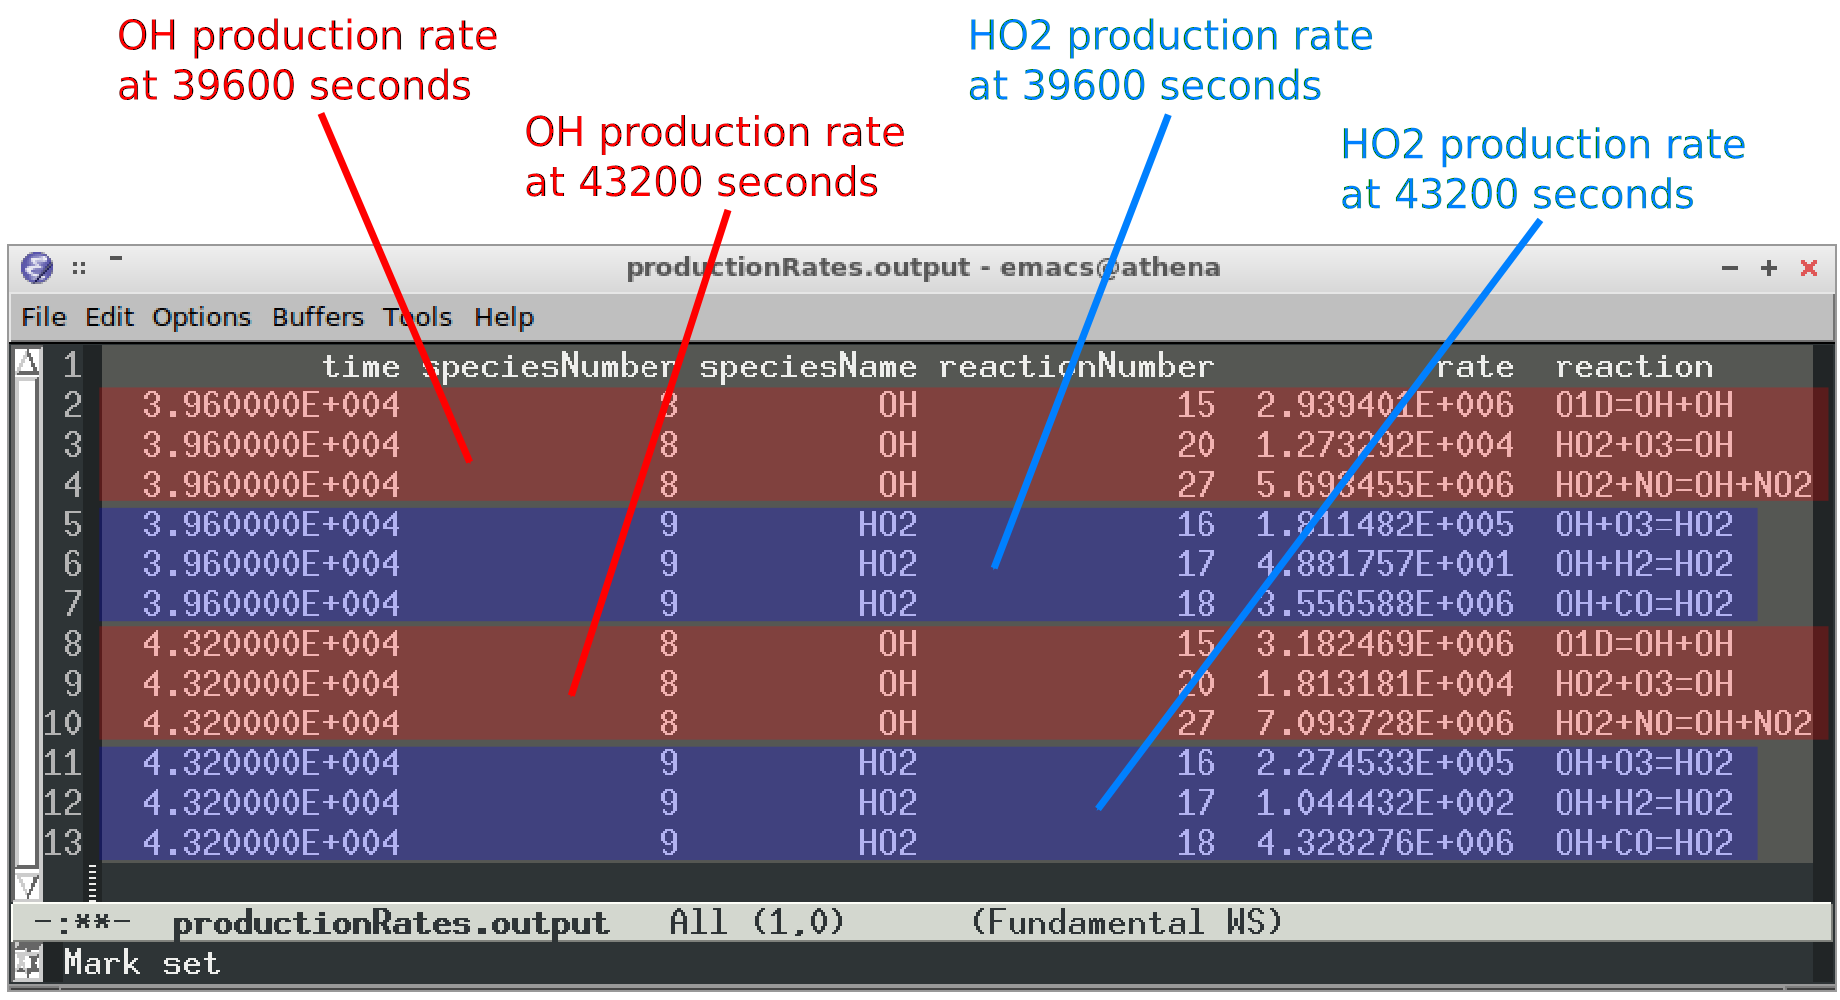
\includegraphics[width=0.95\textwidth]{output-rates.png}
  \caption{Format of the file \texttt{productionRates.output}. The file
    \texttt{lossRates.output} has a similar format.} \label{fig:ropa}
\end{figure}

While the model is running, diagnostic information is printed
to the terminal: this can be redirected to a log file using standard
unix commands. A successfull model run completes with a message
similar to the one shown in Sect.~\ref{sec:install}.

% -----------------------------------------------------------------------------
%
% Copyright (c) 2017 Sam Cox, Roberto Sommariva
%
% This file is part of the AtChem2 software package.
%
% This file is covered by the MIT license which can be found in the file
% LICENSE.md at the top level of the AtChem2 distribution.
%
% -----------------------------------------------------------------------------

\chapter{Model Development} \label{ch:development}

% -------------------------------------------------------------------- %
\section{General Information} \label{sec:general-information}

There are two versions of AtChem2 in the main
\href{https://github.com/AtChem/AtChem2}{github repository}:

\begin{enumerate}
\item Stable version: is indicated by a version number (e.g.,
  \textbf{v1.0}), and can be downloaded from the
  \href{https://github.com/AtChem/AtChem2/releases}{Releases page}.
\item Development version -- i.e. the \texttt{master\ branch}: is
  indicated by a version number with the suffix \texttt{-dev} (e.g.,
  \textbf{v1.1-dev}), and can be downloaded as an
  \href{https://github.com/AtChem/AtChem2/archive/master.zip}{archive
    file} or obtained via \textbf{git} (Sect.~\ref{sec:download}).
\end{enumerate}

AtChem2 is under active development, which means that the
\texttt{master\ branch} is sometimes a few steps ahead of the latest
stable release. Any modification to the code is automatically run
through the \hyperref[sec:test-suite]{Test Suite} before it is merged
into the \texttt{master\ branch}. The Test Suite is designed to ensure
that changes to the code do not cause unintended behaviour or
unexplained differences in the model results, so the development
version is normally safe to use. However, it is recommended to use the
stable version for ``production runs'' and publications since it can
be more easily referenced -- see the discussion about traceability and
reproducibility of computational models in \citet{sommariva_2020}.

Feedback, bug reports, comments and suggestions are welcome: the list
of open issues and known bugs can be found on the related
\href{https://github.com/AtChem/AtChem2/issues}{github page}. The
preferred way to contribute to the development of AtChem2 is to use
\textbf{git}: instructions on how to set up git and submit
contributions can be found on the
\href{https://github.com/AtChem/AtChem2/wiki/How-to-contribute}{wiki}.
The coding guidelines for Fortran are detailed in Sect.\ref{sec:style-guide}.

% -------------------------------------------------------------------- %
\section{Test Suite} \label{sec:test-suite}

AtChem2 uses \href{https://github.com/features/actions/}{GitHub Actions} for
\textbf{continuous integration} testing. This programming approach
ensures that changes to the code do not modify the behaviour and the
results of the software in an unintended fashion. The Test Suite is in
the \texttt{test/} directory and consists of a series of tests and
short model runs that check the model functionality and calculations
against known outputs. The \href{https://codecov.io/}{Codecov} service
is used to verify that the Test Suite covers a significant fraction of
the codebase ($>$90\%) and a wide range of common configurations.

There are four types of tests, which can be executed from the
\maindir\ using the \verb|make| command (note that the
\hyperref[subsec:optional-dependencies]{optional dependencies} need to
be installed):

\begin{itemize}
\item \textbf{Indent} and \textbf{Style} tests: check that the
  indentation and coding style of the Fortran code are consistent with
  the guidelines -- \verb|make indenttest| and \verb|make styletest|.
\item \textbf{Unit} tests: check that individual functions generate
  the expected outputs -- \verb|make unittests|.
\item \textbf{Behaviour} tests: build and run a number of models with
  different configurations and check that they generate the expected
  outputs -- \verb|make tests|.
\end{itemize}

The command \verb|make alltests| runs all the tests in the Test Suite
in succession. Each test outputs the results to the terminal and, in
case of failure, a log file (\texttt{tests/testsuite.log}) is
generated for the indent, style and behaviour tests. If all tests are
successfully passed the following message is printed to the terminal:

\begin{verbatim}
Style test       PASSED
Indent test      PASSED
Tests            PASSED
  (20/20 tests PASSED)
Testsuite PASSED
\end{verbatim}

The Test Suite is automatically run every time a Pull Request (PR) is
created or updated on the main github repository (\texttt{AtChem/AtChem2}).
The Pull Request triggers a build on GitHub Actions which runs the entire
Test Suite on two architectures (Linux and macOS) with one compiler
(GNU \texttt{gfortran}). The CI tester performs the following tasks on
each architecture:

\begin{itemize}
\item Install \texttt{gfortran}, CVODE, and \texttt{numdiff}:
  \begin{itemize}
  \item Linux: use \texttt{apt-get} for \texttt{gfortran},
    \texttt{numdiff}, and \texttt{liplapack-dev} (a dependency of
    CVODE). Install CVODE from source~\footnote{\texttt{apt-get} could
      also be used to install SUNDIALS, but the repository does not
      currently hold CVODE v2.9.}.
  \item macOS: use \texttt{Homebrew} for \texttt{gfortran} and
    \texttt{numdiff}. Install \texttt{cvode} from source.
  \end{itemize}
\item Build and run the example AtChem2 model using the default
  configuration. PASS if it exits with 0.
\item Build and run the indent and style tests. PASS if all tests pass.
\item Build and run the unit tests. PASS if all unit tests pass.
\item Build and run the behaviour tests. PASS if no differences from
  the reference output files are found, otherwise FAIL.
\end{itemize}

Every test must pass to allow the full CI to pass. This is indicated
by the message ``All checks have passed'' on the github PR page. Pull
Requests should only be merged into the \texttt{master\ branch} once
GitHub Actions has completed with passes on both architectures.

\subsection{Adding new unit tests} \label{subsec:adding-new-unit-tests}

The unit tests are in the \texttt{test/unit\_tests} directory and
require the FRUIT optional dependency (which requires Ruby,
Sect.~\ref{subsec:optional-dependencies}). To add new unit tests,
follow the procedure outlined below:

\begin{itemize}
\item The unit test files are called \texttt{*\_test.f90}. If the new
  unit test to be added fits into an existing test file, edit that
  file -- otherwise, create a new test file following the same naming
  pattern. It is suggested that unit tests covering functions from the
  source file \texttt{xFunctions.f90} should be named
  \texttt{x\_test.f90}.
\item The unit test file must contain a module with the same name as
  the file -- i.e. \texttt{x\_test} -- and it must include the
  statement \verb|use fruit|, plus any other required module.
\item The module should contain a number of subroutines with the
  naming pattern \texttt{test\_*}. These subroutines must take no
  arguments and, importantly, must not have any brackets for arguments
  -- subroutine \texttt{test\_calc} is correct, but subroutine
  \texttt{test\_calc()} is wrong.
\item Each subroutine should call one or more assert functions:
  usually, these are \texttt{assert\_equals()}, \texttt{assert\_not\_equals()},
  \texttt{assert\_true()}, \texttt{assert\_false()}. The assert functions
  act as the arbiters of pass or failure of the unit test -- each
  assert must pass for the subroutine to pass, and each subroutine
  must pass for the unit tests to pass.
\item The assert functions have the following syntax:
  \begin{verbatim}
  call assert_true( a == b , "Test that a and b are equal")
  call assert_false( a == b , "Test that a and b are not equal")
  call assert_equals( a, b , "Test that a and b are equal")
  call assert_not_equals( a, b , "Test that a and b are not equal")
  \end{verbatim}
\end{itemize}

It is useful to use the last argument of the assert function as a
\emph{unique} and \emph{descriptive} message. When a unit test fails,
it is highlighted in the FRUIT output summary, and the message of the
assert function is printed. Unique and descriptive messages thus
enable faster and easier understanding of which test has failed, and
perhaps why.

If these steps are followed, calling \texttt{make\ unittests} is
enough to run all the unit tests, including the new ones. To verify
that the new tests have indeed been run and passed, check the output
summary -- there should be a line associated to each of the
\texttt{test\_*} subroutines in each test file.

\subsection{Adding new behaviour tests} \label{subsec:adding-new-behaviour-tests}

Each behaviour test (\texttt{\$TESTNAME}) is contained in its own
subdirectory inside the \texttt{test/tests/} directory. A behaviour
test requires the following files and directory structure:

\begin{verbatim}
|- model
|  |- configuration
|  |  |- $TESTNAME.fac
|  |  |- environmentVariables.config
|  |  |- mechanism.reac.cmp
|  |  |- mechanism.prod.cmp
|  |  |- mechanism.species.cmp
|  |  |- mechanism.ro2.cmp
|  |  |- model.parameters
|  |  |- outputSpecies.config
|  |  |- outputRates.config
|  |  |- photolysisConstant.config    [*]
|  |  |- photolysisConstrained.config [*]
|  |  |- solver.parameters
|  |  |- speciesConstrained.config    [*]
|  |  |- speciesConstant.config       [*]
|  |  |- initialConcentrations.config
|  |- constraints     [**]
|     |- environment/ [**]
|     |- photolysis/  [**]
|     |- species/     [**]
|- output
|  |- reactionRates/
|  |- concentration.output.cmp
|  |- environmentVariables.output.cmp
|  |- errors.output.cmp
|  |- finalModelState.output.cmp
|  |- initialConditionsSetting.output.cmp
|  |- jacobian.output.cmp
|  |- lossRates.output.cmp
|  |- mainSolverParameters.output.cmp
|  |- photolysisRates.output.cmp
|  |- photolysisRatesParameters.output.cmp
|  |- productionRates.output.cmp
|- $TESTNAME.out.cmp
\end{verbatim}

The files marked with \texttt{[*]} and the directories marked with
\texttt{[**]} are optional -- depending on the configuration used in
the test. If present, the directories marked with \texttt{[**]} should
contain the relevant constraint files, according to the corresponding
configuration files in \texttt{model/configuration/} (see
Sect.~\ref{sec:constraints} for details).

The file \texttt{\$TESTNAME.out.cmp} should contain the exact copy of
the expected terminal printout. Each behaviour test is briefly
described in the \texttt{test/tests/INFO.md} file, which should be
updated after a new test is added. New tests added to the
\texttt{test/tests/} directory are automatically picked up by the
\texttt{Makefile} when running \verb|make test| or \verb|make alltests|
from the \maindir.

% -------------------------------------------------------------------- %
\section{Style Guide} \label{sec:style-guide}

In order to make the AtChem2 code more readable and easier to
maintain, the source code should follow a consistent style
(Sect.~\ref{subsec:style-recommendations}). Two Python scripts are used
to check and correct the Fortran code:

\begin{itemize}
\item \texttt{fix\_style.py} edits a Fortran file in-place to make the
  code consistent with the style recommendations.
\item \texttt{fix\_indent.py} works in a similar way, but only looks
  at the indentation level of each line of code.
\end{itemize}

These scripts are in the \texttt{tools/} directory and can be invoked
from the \maindir\ with the following commands:

\begin{verbatim}
python tools/fix_style.py src/filename.f90
python tools/fix_indent.py src/filename.f90
\end{verbatim}

It is important to keep in mind that these scripts are \emph{not
  infallible} and, therefore, it is strongly recommended to always
have a backup of the Fortran file to revert to, in case of wrong
edits. This can be done by passing two arguments to the script instead
of one: the second argument sends the script output to another file,
leaving the original file untouched.

Both scripts are also used in the Test Suite to run the style and
indent tests (Sec.~\ref{sec:test-suite}): each script is run over each
source file and the output is sent to a \texttt{.cmp} file. If the
\texttt{.cmp} file matches the original file, the test passes.

\subsection{Style recommendations} \label{subsec:style-recommendations}

\subsubsection{General principles}

\begin{itemize}
\item All code should be organized in a \textbf{module structure},
  except the main program. There is only one exception: due to a
  complicating factor with linking to CVODE, the functions
  \texttt{FCVFUN()} and \texttt{FCVJTIMES()} are placed within the
  main file \texttt{atchem.f90}.
\item All code should be written in free-form Fortran, and the source
  files should have the extension \texttt{.f90}.
\item Always use two spaces to indent blocks.
\item At the top of each file there should be a header indicating the
  author(s), date, and purpose of the code; if necessary,
  acknowledgements to other contributors should be added.
\item Always comment a procedure with a high-level explanation of what
  that procedure does.
\item There are no specific guidelines for comments, although common
  sense applies and any code within the comments should broadly follow
  the rules below.
\end{itemize}

\subsubsection{Specific recommendations}

\begin{itemize}
\item All \textbf{keywords} should be lowercase, e.g., \texttt{if\
    then}, \texttt{call}, \texttt{module}, \texttt{integer},
  \texttt{real}, \texttt{only}, \texttt{intrinsic}. This includes the
  \texttt{(kind=XX)} and \texttt{(len=XX)} statements.
\item All \textbf{intrinsic} function names should be lowercase, e.g.,
  \texttt{trim}, \texttt{adjustl}, \texttt{adjustr}.
\item The \textbf{relational operators} should use \texttt{$\geq$} and
  \texttt{==} rather than \texttt{.GE.}, \texttt{.EQ.}, and should be
  surrounded by a single space.
\item The \texttt{=} operator should be surrounded by one space when
  used as assignment -- except in the cases of the \texttt{(kind=XX)}
  and \texttt{(len=XX)} statements, where no spaces should be used.
\item The \textbf{mathematical operators} (\texttt{*}, \texttt{-},
  \texttt{+}, \texttt{**}) should be surrounded by one space.
\item Numbers in scientific notation should have no spaces around the
  \texttt{+} or \texttt{-}, e.g., \texttt{1.5e-9}.
\item The names of \textbf{variables} should begin with lowercase,
  while those of \textbf{procedures} (that is, subroutines and
  functions) should begin with uppercase. An exception is
  \textbf{third-party functions}, which should be uppercase. Use
  either CamelCase or underscores to write multiple-word identifiers.
\item All \textbf{modules} should include the \texttt{implicit none}
  statement.
\item All \textbf{variable declarations} should include the
  \texttt{::} notation.
\item The \textbf{dummy arguments} of a procedure should include an
  \texttt{intent} statement in their declaration.
\item The following rules apply to \textbf{brackets}:
  \begin{itemize}
  \item Opening brackets should not have a space before them, except
    for \texttt{read}, \texttt{write}, \texttt{open}, \texttt{close}
    statements.
  \item All \texttt{call} statements and the definitions of all
    procedures should contain one space before the first argument and
    one after the last argument inside the brackets:
    \begin{verbatim}
    call function_name( arg1, arg2 )
    subroutine subroutine_name( arg1 )
    \end{verbatim}
  \item Functions calls and array indices should not have spaces
    before the first argument or after the last argument inside the
    brackets.
  \end{itemize}
\end{itemize}

% -----------------------------------------------------------------------------
%
% Copyright (c) 2017 Sam Cox, Roberto Sommariva
%
% This file is part of the AtChem2 software package.
%
% This file is covered by the MIT license which can be found in the file
% LICENSE.md at the top level of the AtChem2 distribution.
%
% -----------------------------------------------------------------------------

\chapter{Credits and Acknowledgements} \label{ch:credits}

% -------------------------------------------------------------------- %
\section{Credits} \label{sec:credits}

\textbf{AtChem-online} was developed at the
\href{https://www.leeds.ac.uk}{University of Leeds} in 2009-2012 by:

\begin{itemize}
\item Chris Martin
\item Kasia Boro{\'n}ska
\item Jenny Young
\item Peter Jimack
\item Mike Pilling
\end{itemize}

Model evaluation, development of test scenarios and model testing were
done by Andrew Rickard (NCAS) and Monica V{\'a}zquez Moreno (CEAM/EUPHORE).
Technical support was provided by David Waller (University of Leeds).

\textbf{AtChem2} was developed from the \textbf{AtChem-online}
codebase (rev.146) at the \href{https://le.ac.uk}{University of
  Leicester} in 2017-2018 by:

\begin{itemize}
\item Sam Cox
\item Roberto Sommariva (also at \href{https://www.birmingham.ac.uk}{University of Birmingham})
\end{itemize}

\section{Acknowledgements} \label{sec:acknowledgements}

Additional contributions by:

\begin{itemize}
\item Peter Br{\"a}uer
\item Vasilis Matthaios
\item Beth Nelson
\item Mike Newland
\item Marios Panagi
\item Robert Woodward-Massey
\end{itemize}

Special thanks to Harald Stark (University of Colorado-Boulder, USA)
for providing data to test the photolysis rates subroutines. And to
J.-F. Doussin (Universit{\'e} Paris-Est Cr{\'e}teil, France). Bill
Bloss and Paul Monks

% -------------------------------------------------------------------- %
\section{Funding} \label{sec:funding}

Funding has been provided at different stages by:

\begin{itemize}
\item \href{https://www.eurochamp.org/}{EUROCHAMP project}.
\item Natural Environment Research Council (\href{https://nerc.ukri.org/}{NERC}).
\item University of Leicester Research Software Engineering Team (ReSET).
\item NCAS
\end{itemize}


\bibliographystyle{abbrvnat}
\bibliography{References}
\addcontentsline{toc}{chapter}{References}

\end{document}
%    rates output and reaction rates output can't be zero in config
